%-*- coding: UTF-8 -*-
%%%%%%%%%%%%%%%%%%%%%%%%%%%%%%%%%%%%%%%%%%%%%%%%%%%%%%%%%%%%%%%%%%%%%%%%%%%%%%%%
%          ,
%      /\^/`\
%     | \/   |                CONGRATULATIONS!
%     | |    |             SPRING IS IN THE AIR!
%     \ \    /                                                _ _
%      '\\//'                                               _{ ' }_
%        ||                     hithesis v3                { `.!.` }
%        ||                                                ',_/Y\_,'
%        ||  ,                   dustincys                   {_,_}
%    |\  ||  |\          Email: yanshuoc@gmail.com             |
%    | | ||  | |            https://yanshuo.name             (\|  /)
%    | | || / /                                               \| //
%    \ \||/ /       https://github.com/dustincys/hithesis      |//
%      `\\//`   \\   \./    \\ /     //    \\./   \\   //   \\ |/ /
%     ^^^^^^^^^^^^^^^^^^^^^^^^^^^^^^^^^^^^^^^^^^^^^^^^^^^^^^^^^^^^^^
%%%%%%%%%%%%%%%%%%%%%%%%%%%%%%%%%%%%%%%%%%%%%%%%%%%%%%%%%%%%%%%%%%%%%%%%%%%%%%%%
\documentclass[fontset=fandol,type=bachelor,campus=harbin]{hithesisbook}
% 此处选项中不要有空格
%%%%%%%%%%%%%%%%%%%%%%%%%%%%%%%%%%%%%%%%%%%%%%%%%%%%%%%%%%%%%%%%%%%%%%%%%%%%%%%%
% 必填选项
% type=doctor|master|bachelor|postdoc
%%%%%%%%%%%%%%%%%%%%%%%%%%%%%%%%%%%%%%%%%%%%%%%%%%%%%%%%%%%%%%%%%%%%%%%%%%%%%%%%
% 选填选项(选填选项的缺省值已经尽可能满足了大多数需求,除非明确知道自己有什么
% 需求)
% campus=shenzhen|weihai|harbin
%   含义:校区选项,默认harbin
% glue=true|false
%   含义:由于我工规范中要求字体行距在一个闭区间内,这个选项为true表示tex自
%   动选择,为false表示区间内一个最接近版心要求行数的要求的默认值,缺省值为
%   false。
% tocfour=true|false
%   含义:是否添加第四级目录,只对本科文科个别要求四级目录有效,缺省值为
%   false
% fontset=windows|mac|ubuntu|fandol|adobe
%   含义:设置字体,默认情况会自动识别系统,然后设置字体。后两个是开源字体,自行
%   下载安装后设置使用。windows是中易字库,窝工默认常用字体,绝对没毛病。mac和
%   ubuntu 默认分别是华文和思源字库,理论上用什么字库都行。后两种开源字库的安装
%   方法到谷歌上百度一下什么都有了。Linux非ubuntu发行版、非x86架构机器等如何运行
%   可到github issue上讨论。
% tocblank=true|false
%   含义:目录中第一章之前,是否加一行空白。缺省值为true。
% chapterhang=true|false
%   含义:目录的章标题是否悬挂居中,规范中要求章标题少于15字,所以这个选项
%   有无没什么用,除了特殊需求。缺省值为true。
% fulltime=true|false
%   含义:是否全日制,缺省值为true。非全日制如同等学力等,要在cover中设置类
%   型,封面中不同格式
% subtitle=true|false
%   含义:论文题目是否含有副标题,缺省值为false,如果有要在cover中设置副标
%   题内容,封面中显示。
% newgeometry=one|two|no
%   含义:规范中的自相矛盾之处,版芯是否包含页眉页脚,旧方法是按照包含页眉
%   页脚来设置。该选项是多选选项,如果设置为no,则版新为旧模板的版芯设置方法,
%   如果设置该选项one或two,分别对应两种页眉页码对应版芯线的相对位置。第一种
%   是严格按照规范要求,难看。第二种微调了页眉页码位置,好一点。默认two。
% debug=true|false
%   含义:是否显示版芯框和行号,用来调试。默认否。
% openright=true|false
%   含义:博士论文是否要求章节首页必须在奇数页,此选项不在规范要求中,按个
%   人喜好自行决定。 默认否。注意,窝工的默认情况是打印版博士论文要求右翻页
%   ,电子版要求非右翻页且无空白页。如果想DIY(或身不由己DIY)在什么地方右
%   翻页,将这个选项设置为false,然后在目标位置添加`\cleardoublepage`命令即
%   可。
% library=true|false
%   含义:是否为提交到图书馆的电子版。默认否。注意:如果设置成true,那么
%   openright选项将被强制转换为false。
% capcenterlast=true|false
%   含义:图题、表题最后一行是否居中对齐(我工规范要求居中,但不要求居中对
%   齐),此选项不在规范要求中,按个人喜好自行决定。默认否。
% subcapcenterlast=true|false
%   含义:子图图题最后一行是否居中对齐(我工规范要求居中,但不要求居中对齐
%   ),此选项不在规范要求中,按个人喜好自行决定。默认否。
% absupper=true|false
%   含义:中文目录中的英文摘要在中文目录中的大小写样式歧义,在规范中要求首
%   字母大写,在work样例中是全大写。该选项控制是否全大写。默认否。
% bsmainpagenumberline=true|false
%   含义:由于本科生论文官方模板的页码和页眉格式混乱,提供这个选项自定义设
%   置是否在正文中显示页码横线,默认否。
% bsfrontpagenumberline=true|false
%   含义:由于本科生论文官方模板的页码和页眉格式混乱,提供这个选项自定义设
%   置是否在前文中显示页码横线,默认否。
% bsheadrule=true|false
%   含义:由于本科生论文官方模板的页码和页眉格式混乱,提供这个选项自定义设
%   置是否显示页眉横线,默认显示。
% splitbibitem=true|false
%   含义:参考文献每一个条目内能不能断页,应广大刀客要求添加。默认否。
% newtxmath=true|false
%   含义:数学字体是否使用新罗马。默认是。
% chapterbold=true|false
%   含义:本科生章标题在目录和正文中是否加粗
% engtoc=true|false
%   含义:非博士生需要添加英文目录的,手动添加,如果是博士,此开关无效
% zijv=word|regu
%   含义:字距设置为规范规定33个字还是word中34个字。默认regu。
%%%%%%%%%%%%%%%%%%%%%%%%%%%%%%%%%%%%%%%%%%%%%%%%%%%%%%%%%%%%%%%%%%%%%%%%%%%%%%%%
\usepackage{hithesis}

\graphicspath{{figures/}}

\begin{document}
\frontmatter
% !Mode:: "TeX:UTF-8"

\hitsetup{
    %******************************
    % 注意:
    %   1. 配置里面不要出现空行
    %   2. 不需要的配置信息可以删除
    %******************************
    %
    %=====
    % 秘级
    %=====
    statesecrets={公开},
    natclassifiedindex={TM301.2},
    intclassifiedindex={62-5},
    %
    %=========
    % 中文信息
    %=========
    ctitleone={基于移动大数据的},%本科生封面使用
    ctitletwo={用户职住特征分析},%本科生封面使用
    ctitlecover={基于移动大数据的用户职住特征分析},%放在封面中使用,自由断行
    ctitle={基于移动大数据的用户职住特征分析},%放在原创性声明中使用
    % csubtitle={一条副标题}, %一般情况没有,可以注释掉
    cxueke={管理学},
    csubject={信息管理与信息系统},
    caffil={经济与管理学院},
    cauthor={谢三山},
    csupervisor={叶强教授},
    cassosupervisor={刘旭东}, % 副指导老师
    % ccosupervisor={某某某教授}, % 联合指导老师
    % 日期自动使用当前时间,若需指定按如下方式修改:
    %cdate={超新星纪元},
    cstudentid={1171000514},
    % cstudenttype={同等学力人员}, %非全日制教育申请学位者
    cnumber={no1171000514}, %编号
    cpositionname={哈铁西站}, %博士后站名称
    cfinishdate={20XX年X月---20XX年X月}, %到站日期
    csubmitdate={20XX年X月}, %出站日期
    cstartdate={3050年9月10日}, %到站日期
    cenddate={3090年10月10日}, %出站日期
    %(同等学力人员)、(工程硕士)、(工商管理硕士)、
    %(高级管理人员工商管理硕士)、(公共管理硕士)、(中职教师)、(高校教师)等
    %
    %
    %=========
    % 英文信息
    %=========
    etitle={Research on key technologies of partial porous externally pressurized gas bearing},
    esubtitle={This is the sub title},
    exueke={Engineering},
    esubject={Computer Science and Technology},
    eaffil={\emultiline[t]{School of Mechatronics Engineering \\ Mechatronics Engineering}},
    eauthor={Yu Dongmei},
    esupervisor={Professor XXX},
    eassosupervisor={XXX},
    % 日期自动生成,若需指定按如下方式修改:
    edate={December, 2017},
    estudenttype={Master of Art},
    %
    % 关键词用“英文逗号”分割
    ckeywords={大数据, 职业, 家庭, 用户画像分析},
    ekeywords={bigdata, occupation, family, user potrait analysis},
}

\begin{cabstract}
    摘要的字数(以汉字计),硕士学位论文一般为500 $\sim$ 1000字,博士学位论文为1000 $\sim$ 2000字,
    均以能将规定内容阐述清楚为原则,文字要精练,段落衔接要流畅。摘要页不需写出论文题目。
    英文摘要与中文摘要的内容应完全一致,在语法、用词上应准确无误,语言简练通顺。
    留学生的英文版博士学位论文中应有不少于3000字的“详细中文摘要”。

    关键词是为了文献标引工作、用以表示全文主要内容信息的单词或术语。关键词不超过 5
    个,每个关键词中间用分号分隔。(模板作者注:关键词分隔符不用考虑,模板会自动处
    理。英文关键词同理。)
\end{cabstract}

\begin{eabstract}
    An abstract of a dissertation is a summary and extraction of research work
    and contributions. Included in an abstract should be description of research
    topic and research objective, brief introduction to methodology and research
    process, and summarization of conclusion and contributions of the
    research. An abstract should be characterized by independence and clarity and
    carry identical information with the dissertation. It should be such that the
    general idea and major contributions of the dissertation are conveyed without
    reading the dissertation.

    An abstract should be concise and to the point. It is a misunderstanding to
    make an abstract an outline of the dissertation and words ``the first
    chapter'', ``the second chapter'' and the like should be avoided in the
    abstract.

    Key words are terms used in a dissertation for indexing, reflecting core
    information of the dissertation. An abstract may contain a maximum of 5 key
    words, with semi-colons used in between to separate one another.
\end{eabstract}
 % 封面
\makecover
\begin{denotation}
\begin{table}[h]%此处最好是h
\caption{国际单位制中具有专门名称的导出单位}
\vspace{0.5em}\centering\wuhao
\begin{tabular}{ccccc}
\toprule[1.5pt]
量的名称&单位名称&单位符号&其它表示实例\\
\midrule[1pt]
频率&赫[兹]&Hz&s-1\\
\bottomrule[1.5pt]
\end{tabular}
\end{table}
\end{denotation}
%物理量名称表,符合规范为主,有要求添加
\tableofcontents %目录
\mainmatter
% !Mode:: "TeX:UTF-8"

\chapter{绪论}

\section{研究课题的来源、背景和意义}

本研究课题来源于哈尔滨工业大学和中国移动联合实验室承接的基于黑龙江省移动用户数据开展多方面的研究和分析。本研究需要解决的问题是通过移动提供的数据,对哈尔滨市用户的职业、家庭特征进行分析,绘制出用户画像,为后续精准营销、城市规划等研究打下数据基础。

\section{国内外与课题相关研究领域的研究进展及成果}

\subsection{大数据及其相关理论和应用的发展概况}
\label{sec:bd_dev}

全球互联网时代的到来,不管是早期的个人电脑、移动电话,甚至是目前发展势头正盛的各种接入互联网的设备形成的物联网,虽然带给人们越来越多的便携性,但各方面人士对偌大的全球性网络中产生的数据提出相当多的问题。除了个人隐私、数据归属等使用权以及相关法律层面的问题,开发人员不能逃避的一个重要问题则是超大规模数据的存储、处理和查询。

根据国际数据公司(IDC,International Data Corporation)的预测\cite{data_count},由于 5G 的商用化在中国国内逐渐铺开,企业和用户的设备产生的数据将会成为中国数据的主流,数据量和数据市场将产生跨越式增长,在 2023 年左右达到 40ZB ($1ZB \approx 10^{12}GB$)。

飞速增长的数据量,无论单台计算机的存储能力、计算速度达到何种水平,在数以 PB 计的数据量面前,都不足以应对。同时,单机的价格相对于其性能并不是线性增加的,昂贵的单机服务器使团体或者公司无法负担处理如此庞大数据量的成本,二十世纪初的大数据也只能被丢弃。

首先解决该问题的是谷歌,2003 年谷歌发表了三篇技术论文\cite{gfs},分别是解决了存储大规模数据的 GFS(Google File System,谷歌文件系统),解决了大规模计算的 MapReduce 方法,以及解决了实时查询的 BigTable 系统。之后雅虎公司推出了 Hadoop 平台及其生态,被 Apache Software Foundation 公司引入开源应用。 其中,最有价值的 GFS 相关的论文使得 HDFS(Hadoop Distributed File System,Hadoop 分布式文件系统)的开源实现成为了目前绝大部分大数据平台的基石。

\begin{figure}[htpb]
    \centering
    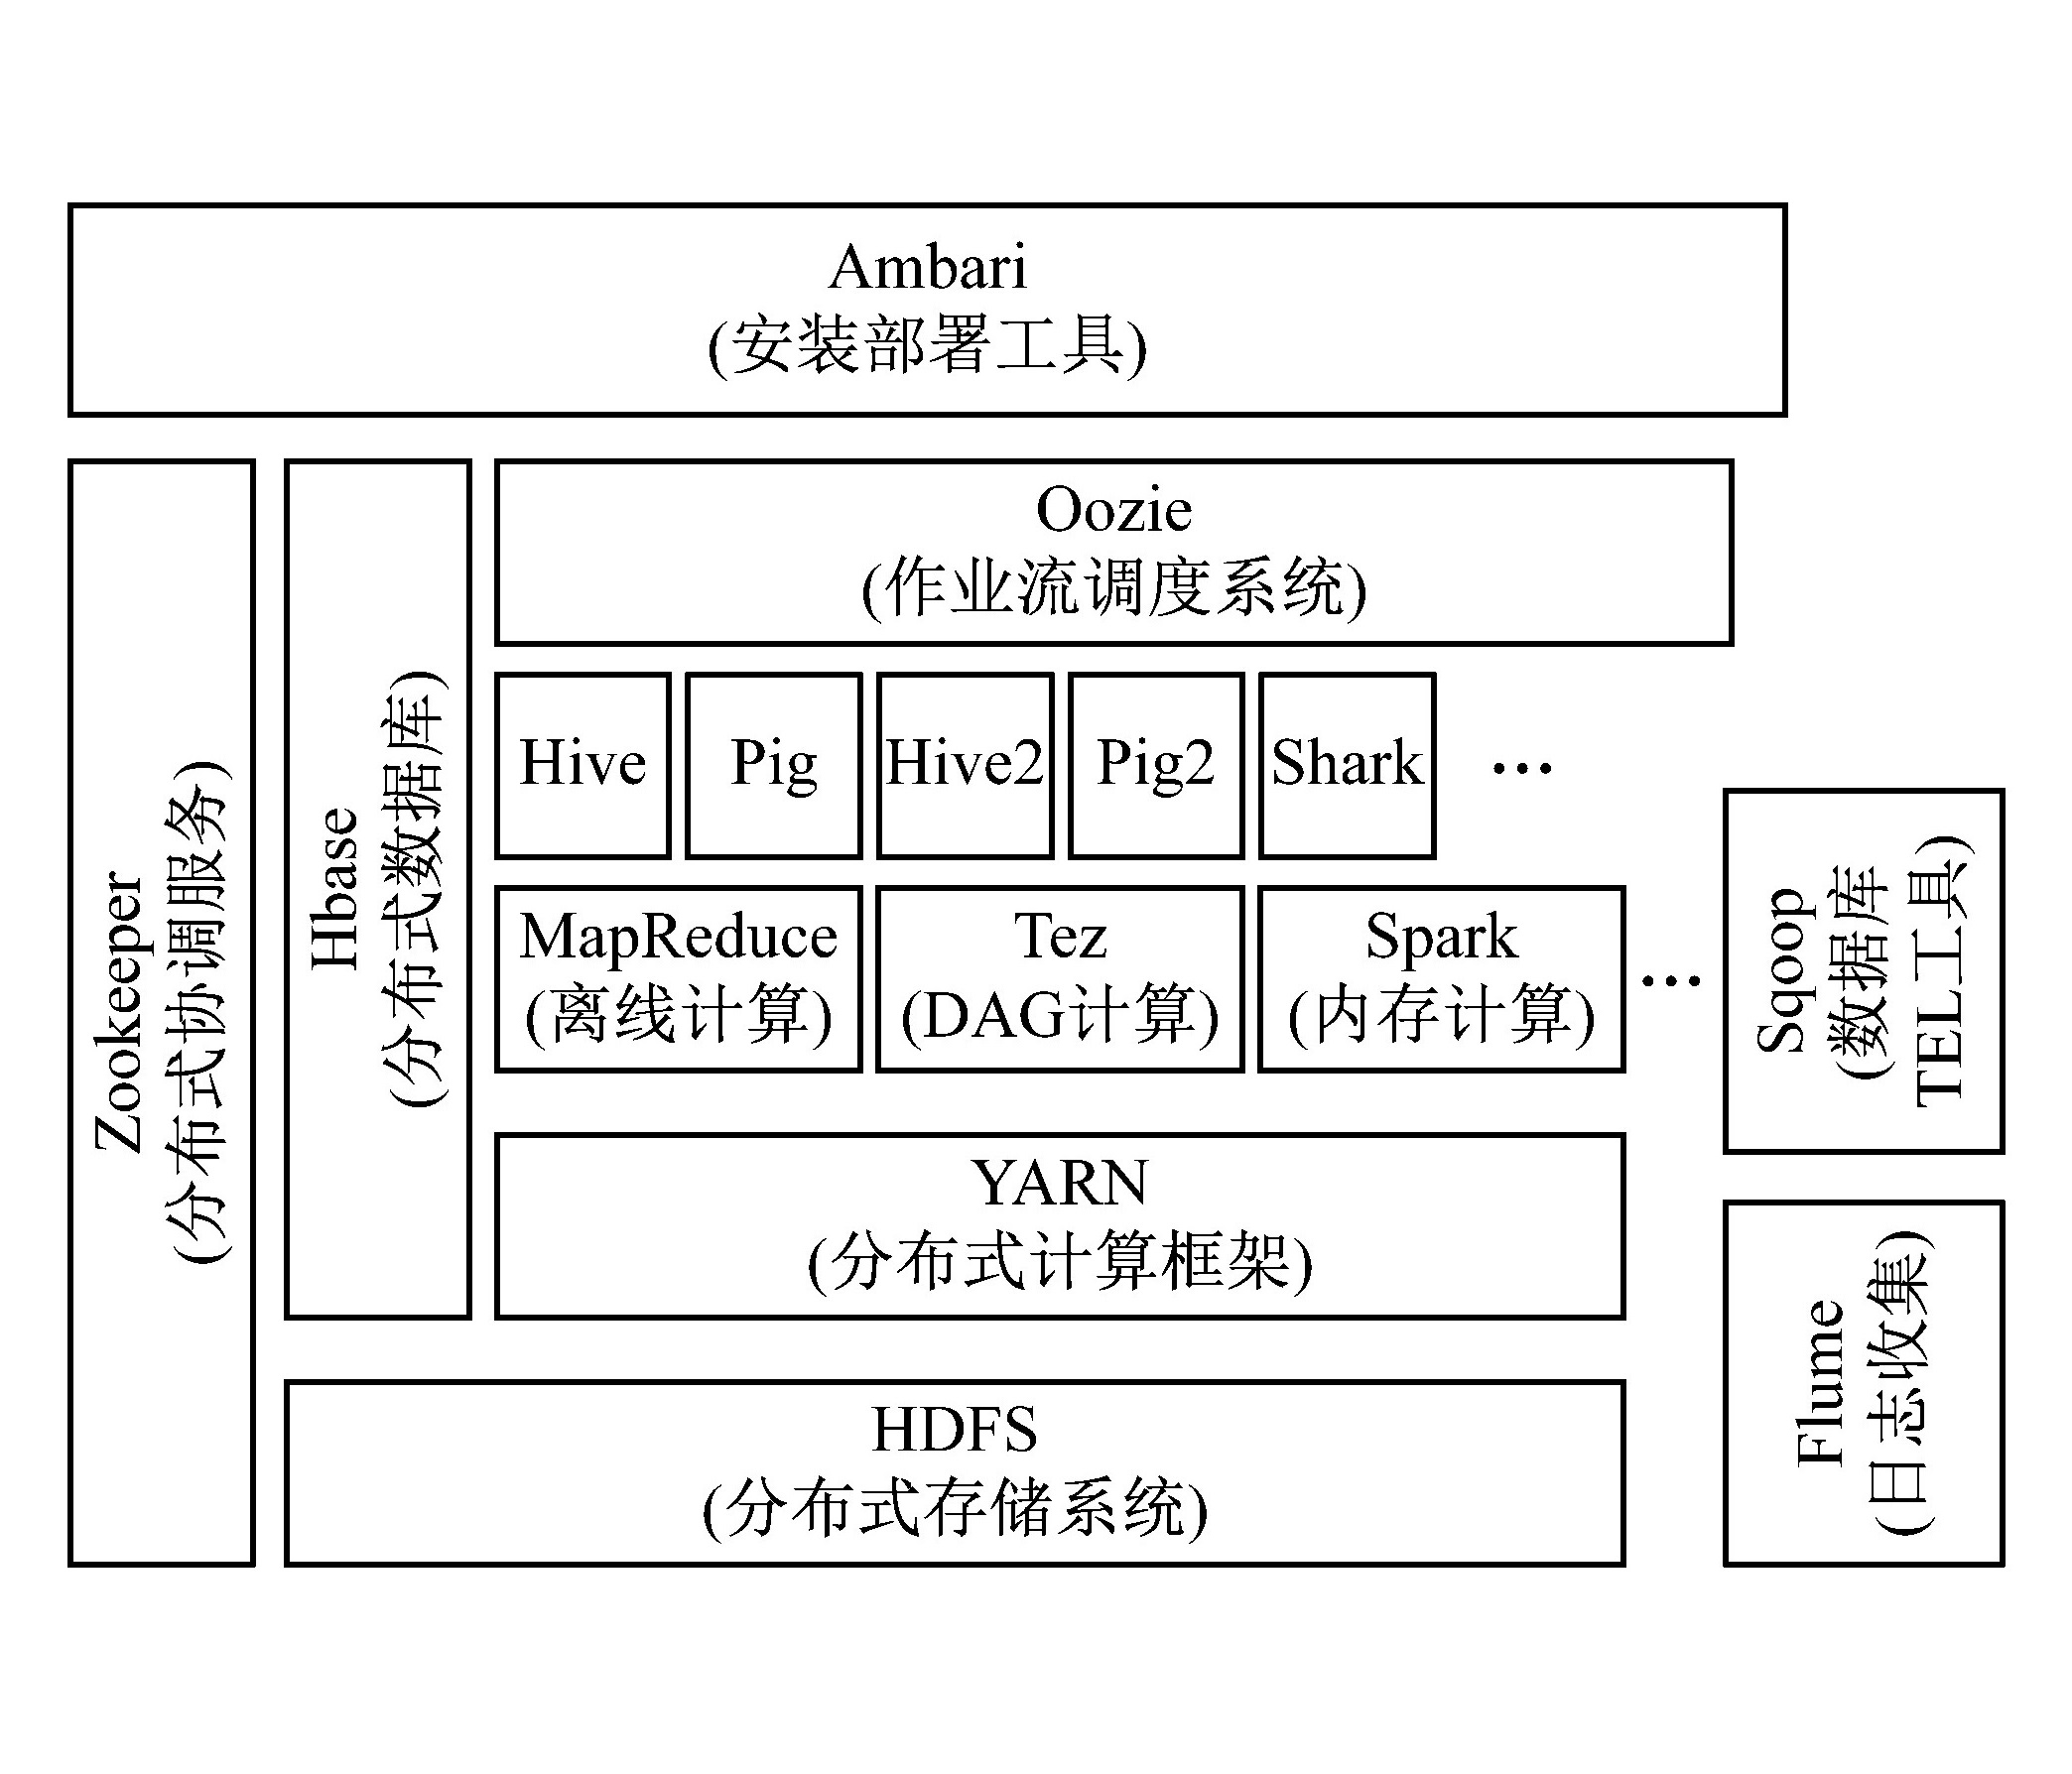
\includegraphics[width = 0.8\textwidth]{hadoop.jpg}
    \caption{Hadoop 生态系统}
    \label{fig:hadoop}
\end{figure}

如图 \ref{fig:hadoop} 所示,最底层的 HDFS 分布式文件存储系统是整个大数据领域的基础,通过切分超大文件,实现了一个多机保存、备份以及高容错的大数据文件系统。HDFS 只上的是 Yarn(全称 Yet Another Resource Manager),主要由于 Hadoop 1.0 版本中的重大架构缺陷,导致任务调度系统(JobTracker)承担了太多诸如资源调度、异常监控、接受任务等不同且复杂的任务,于是行业将 JobTrakcer 的任务拆分开来,形成了建立在 HDFS 上的新的调度系统,能够兼容更多的计算框架,如本研究使用的 Spark 以及同样用 DAG 优化的 Tez 等。

MapReduce 则是一种计算模型,通过一次 Map 操作生成 key-value 键值对,以及第二次 Reduce 操作对所有键值对进行规约,得到最终的结果。而 MapReduce 如此暴力的实现方法被数据库领域的专家 David J. DeWitt\cite{mr_back} 在一篇著名论文 \emph{MapReduce: A Major Step Backwards} 中指责谷歌在大数据的计算上即 MapReduce 方法放弃了数据库领域中的优秀理论和方案,选择了简单粗暴的解决办法。不久,加州大学伯克利学院的 AMP 实验室则推出取 MapReduce 和数据库中精华的 Spark 平台,通过 DAG(有向无环图)解决了多次机器学习、聚类算法中多次迭代的麻烦问题,以及稳定的 Spark Streaming,MLlib 等拳头产品,使 Spark 平台及其套件,成为众多公司的选择。

\begin{figure}[htpb]
    \centering
    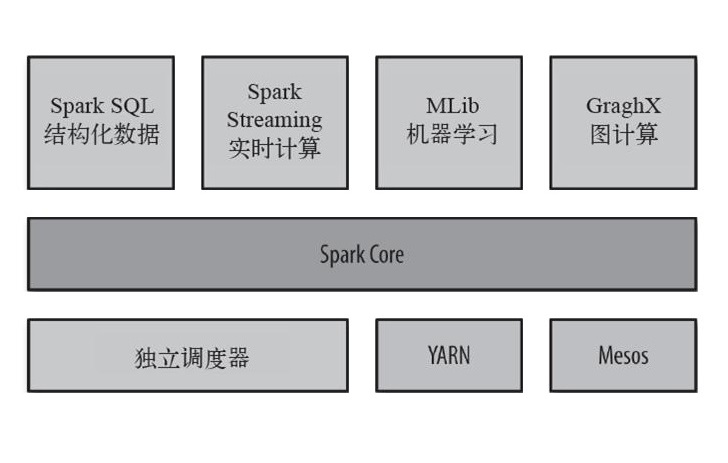
\includegraphics[width = 0.8\textwidth]{spark.jpg}
    \caption[fig:spark]{Spark 生态系统}
    \label{fig:spark}
\end{figure}

如图 \ref{fig:spark} 所示,整个 Spark 生态系统中的核心是 Spark Core,从基于 HDFS 的 YARN 框架、HBase、Hive 数据库等中读取数据,通过独立调度器(Standalone)、YARN 和 Mesos 调度任务(Job),然后完成 Spark 程序,或者通过 spkar-shell/spark-submit 等命令行工具,批量运行或提交任务,再利用基于 Spark Core 的 Spark Stream 完成实时计算、MLLib 实现机器学习以及 GraghX 进行图形计算提高程序运行速度。

除此之外,与只推荐用 Java 编写 MapReduce 程序不同,Spark 能够和多种动态或静态语言配合,如 Python、Scala、Java,甚至能够启用 spark-shell 命令行工具,使用 Scala 语言进行交互式查询,灵活便捷。Spark 还支持更复杂的操作,除开类似 MapReduce 的固定的生成 key-value 键值对的方法,Spark 基于 RDD 模型(Resilient Distributed Datasets,抽象弹性分布式数据集),只需要承担非常小的代价,就能实现如 SQL 中的 join、union 等高阶方法,以及流式查询功能。

\subsection{手机信令数据与职住特分析的相关理论和发展概况}

2020 年 9 月,中国互联网络信息中心(CNNIC)第 46 次发布了《中国互联网络发展状况统计报告》\cite{2020_mobile},截止 6 月底,中国已经形成了 9.4 亿规模的网民群体,移动互联网用户规模更是达到了 13.19 亿人,同时“中华人民共和国国民经济和社会发展第十三个五年规划纲要”中首次明确指出 2020 年的互联网普及率计划,要将移动宽带的普及率提升到 85\%,如此庞大的用户数量,必然会产生超大规模的用户数据,客户在日常的手机使用中,会产生诸如基站连接记录、手机应用流量使用记录、点对点通话记录、短信记录等。

其中,用户手机接受信号产生的基站连接记录的数据成为一个重点分析对象,连接数据能够模糊推断出用户的位置,根据这一点,2017 年孔扬鑫\cite{kong_people}采用了轨迹行为特征的判定算法,基于 MapReduce 分布式计算模型,基于用户的基站连接数据,分析基站连接的消失点、消失时长、用户停留点、用户工作地点与家庭住址的平均距离,计算出用户进出城的人口流动的统计数据,再基于基站与县区之间的关系,判断用户的通勤起终点所属区域,最终得到用来反映城镇间、工作地居住地间的人口流动的状态转移序列。

由于城区的范围都比较大,因为基站的覆盖面积广而导致位置的推算的误差并不能显著的影响用户所处城镇的结果。但如果需要精确到城区内部的定位,或者对用户未来位置的推断,就必须要把基站范围导致的误差考虑在内。北京邮电大学 2019 年刘奕杉\cite{liu_pos_forecast}则是基于用户连接基站的记录产生的状态转移序列,构建了位点转移的语义序列,再利用 TS-RNN(Three-layer Symmetircal Recurrent Neural Network,三层对称卷积神经网络)提取出转移特征值,实现了更精准的用户活动区域获取以及位置预测。

常在春\cite{chang_job_space}在延庆区职住空间关系分析一文中同样利用 Spark 大数据平台,首先对延庆地区的手机信令数据做一个初步筛选,主要针非过境、常驻、非固定设备用户的工作以及居住地位置的分析,然后使用核密度法得到多个工作地和居住地对应的基站的信息,最终实现用户对工作地点及居住地点的信息推算,并且对延庆区的通勤、工作地使用情况、居住地使用情况等进行描述和分析。

\subsection{城市功能区与用户行为目的和职住特征分析研究进展及成果}
\label{sec:city_dist}

需要分析用户的职业居住的特征分析,就必然不能绕开对用户所处位置的功能语义分析,即用户处于什么目的而移动到该区域。为了能够大致描述用户目的,就需要对城市进行功能区划分。由文献\cite{yang_beijing_district}可知,杨振山等人融合北京市移动电话信令数据以及网络地图 API 提供的 POI(Point of Interest,兴趣点),通过计算单位数量 POI 的人口密度、标准化的单位面积 POI 密度以及类内散度矩阵等特征,对栅格化后的北京市推断所有区块的主导功能类型,得到如北京市功能区比率分布,居住和餐饮、娱乐、服务等工作区块分布特点,以及区块的日夜活跃等特点。

除了对城市进行栅格化城区对每个区块进行分析,还有根据城市主要路网对市区进行一个大致上的划分,福建农林大学毋亭在对泉州市\cite{quanzhou}按照路网信息划分出不规则的网格作为研究单元,同时提出按照多个属性如群众对区域类型的认知度(如对大学的认知度较高、对一般商店认知度较低)、该类型覆盖的面积对区块进行权重赋值,基于该种划分和权重法,再加上核密度估计法,完成对不同功能区的识别和划分,最后通过对泉州市地图进行对比,验证准确率。

本文研究用户的职住画像,需要根据城市中职住区域的分布进行参数上的调整,文献\cite{wang_beijing}对北京市的职住空间分布进行定量的研究,通过分析北京市三十余天一亿多条的基站的链接数据,根据北京市的路网结构情况,综合运用职住偏离度、空间错误指数和职住分离率等特征,研究城市功能区分布规律和匹配特点,为本研究对哈尔滨市的研究提供了参考。

\subsection{大数据下的职住空间聚类算法的分析和改进}

本研究需要对城市的功能区进行聚类,得到用户移动语义,针对哈尔滨市 67 万余条城市兴趣点信息,需要一个高效、准确的聚类算法。如章节 \ref{sec:bd_dev} 所言,基于 Spark Core 这个核心,以及拆分成不同组件的调度器、Mesos 等结构,Spark 能够灵活的提供非常多种无监督聚类以及有监督的机器学习等操作。比如 Spark MLLib 库中提供的 K-Means 算法,通过基于 HDFS 的 Yarn 框架,读取分布式数据,采用类似 Map 的方法生成若干对键值对,Spark Core 再将这些键值对分配到各个节点上,分布式地完成 K-Means 算法,该算法充分利用了 Spark 的高弹性分布式数据集,在高扩展、速度快的条件下,完成多种无监督聚类算法。

文献\cite{zhang_poi},东北大学张景奇等人指出,中国 2010 年到 2019 年截止,知网上有 625 篇关于 POI 兴趣点数据研究的文章,特别是在 2017 年之后发生了爆炸式的增长,而关于 POI 兴趣点的分析方法主要是空间自相关分析、核密度估计以及 DBSCAN 聚类算法。作者的研究表明,兴趣点大数据对城市功能区布局、空间结构以及发展规律的分析都起到一个非常重要的影响。

比如文献\cite{shao_jiejing}就通过背景和上海的兴趣点大数据以及不同的聚类算法,分析北京市和上海市的街道元素,从而得到两市的城市舒适度评价。文献通过路网数据将城市进行语义上的分隔,通过街景元素的可视数量的占比加上 K-Means 聚类分析,将街景分成 29 类并进行相关性分析以及舒适度评价。利用路网数据进行语义分割加上 K-Means 街景分类为本研究的街区分类提供了聚类路线上的参考。

不过本研究的街区划分颗粒度较细,POI 兴趣点的数量较多,使用一般的 Kmeans 聚类算法在时间复杂度上不够优秀,需要寻找优化方法。比如文献\cite{li_minibatch}中,为了提高室内 WLAN 定位的算法性能和准确度,希望通过先聚类再采用 XGBoost 分类算法确定准确位置,为了解决超大规模数据量的问题,文献采用大数据优化的 Minibatch K-Means 聚类算法,降低了数据维数、提高了运算速度的同时,仍然保持了较高的准确率,不失为一个大数据下的聚类优化算法。

\subsection{基于手机信令的用户特征画像分析相关研究进展及成果}

文献\cite{wang_huaxiang}没有着眼于兴趣点驻留偏好,而是通过手机信令数据,刻画出用户的高聚集点,刻画出两点一线、双核心、均匀分布等轨迹类型,再根据用户的其他特征,描述和推测用户的职业类型(如学生、退休老人、技术工种等)、爱好属性,以及年龄层分布等相关信息。文献中值得借鉴的方面,包括数据的预处理,作者首先对原始数据进行均匀间隔采集处理、清楚无效和重复数据、分隔时间段,然后基于 DBSCAN 聚类算法改进出一种高簇聚类法得到用户的如居住点、工作地、娱乐场所等核心点。

除了基站连接数据的应用,文献\cite{zheng_game}中利用游戏类 APP 流量数据与其他 APP 流量数据的比率,同时处理用户的短信费用、流量套餐极其费用以及手机连接流量时发送的请求推算出手机的大致平台,通过上述处理后的数据,划分出不同年龄层、不同消费等级、不同的消费行为以及不同的消费心理等,细分用户群,准确把握客户价值从而实现精确营销。其中对不同 APP 相关数据运用对本研究处理用户 APP 流量数据的处理有一定的引导和启发效果。

\subsection{存在的不足或有待深入研究的问题}
\label{sec:buzu}

章节 \ref{sec:city_dist} 中提到了基于路网的城市区块划分,如文献 \cite{xue_liaoning_dist} 中以辽宁省本溪市为例,配合核密度法、公众认知度以及区块大小等因素推算出城市功能区分类,如图 \ref{fig:liaoning}。但是路网的颗粒度太粗的同时,一些区块如小学校、商场等建筑,并没有用街道去划分界限,导致并不能够较为准确地判断该区域的功能区类型。 

\begin{figure}[htpb]
    \centering
    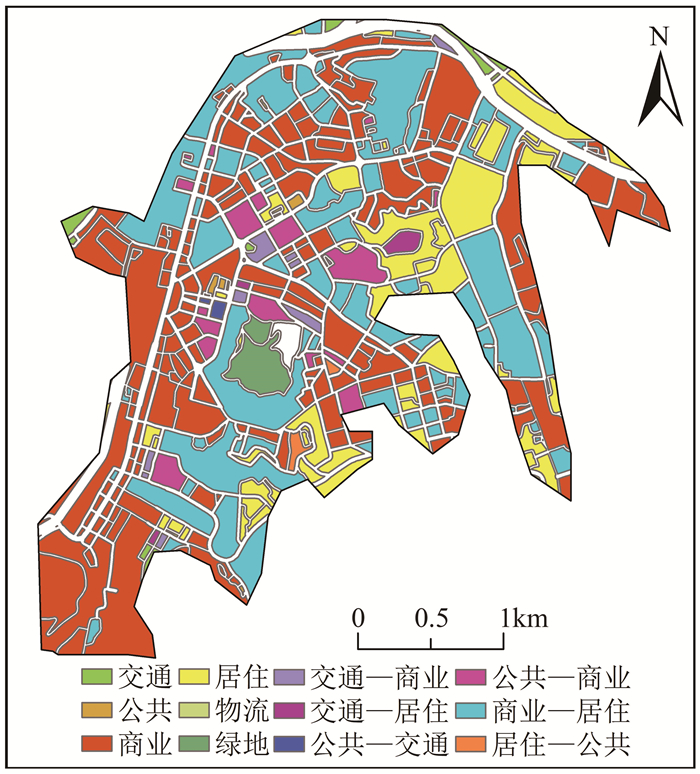
\includegraphics[width = 0.5\textwidth]{liaoling_dist.jpg}
    \caption{辽宁省本溪市功能区分布图}
    \label{fig:liaoning}
\end{figure}

如果采用文献\cite{yang_beijing_district}的中提到的的通过栅格化城市来描述区块的类别,虽然可以在较细颗粒度的情况下分析功能区,但是同样需要注意的是,该方法需要考验研究人员对栅格长宽的确定,不同大小的栅格以及栅格兴趣点 POI 的数据量都会称为影响区块分类的因素。

上面提到的文献中,描述的用户画像多为工作地、居住地、通勤时间等交通、城区规划方向的标签,而缺少对用户是否有工作、工作时长、是否经常加班、使用 APP 偏好等画像的分析,这些都是有待本研究深入研究的问题。

\section{本课题的主要研究内容概述}

\subsection{数据分析与可用性判断}

本研究首先要对中国移动提供的数据进行统一的描述与判断,比如用户与基站的连接数据,每天有多少条用户,用户唯一标识符使用手机号码还是 ICCID(Integrate Circuit Card Identity,集成电路卡识别码即手机 SIM 卡卡号),连接时间的数据类型,字符串或是到 1970 年 1 月 1 日零点的毫秒数等,都需要研究人员仔细分析、做下标记,为之后的研究和处理提供数据轮廓。

同时提取重要的信息表,比如研究用户 APP 偏好画像时,用户 APP 使用数据表和 APP 的描述信息表(如类别,名称,唯一标识符等)都是关键数据,需要认真筛选并且做出数据流向图为数据的分析开发奠定基础。

\subsection{大数据下 K-Means 聚类方法的分析和优化}

由于 K-Means 的时间复杂度为 $O(KNTD)$,K 表示聚类数量,N 表示被聚类元素数量,T 表示迭代次数,D 表示距离的计算复杂度,具体为样本的特征数量,总体来说是关于被聚类元素的总数量的时间复杂度。为了平衡执行速度和聚类效果,本研究会比较两种 K-Means 优化算法,K-Means++ 和 Minibatch K-Means,从中选出一个各方面均衡的聚类优化方法。

\subsection{哈尔滨市栅格化处理以及对栅格化后的街区类型分析}
\label{sec:xu:block_type}

综合章节 \ref{sec:buzu} 中提到诸多因素,本研究选择颗粒度更小的栅格化城市处理方式。首先通过爬虫程序获取哈尔滨市区的兴趣点信息表,然后按照不同的标准对城市进行栅格化处理。对于每次栅格化后的城市,根据每一格中 POI 兴趣点的数量和类型,建立不同的模型来表示这一格中的兴趣点分布情况,接着做一次 K-Means 聚类分析,得到哈尔滨市城市功能区类型的聚类结果。

对于每一次聚类结果,对比哈尔滨市真实的城市地图,分析和判断聚类结果的准确性,调整栅格的长宽,以及描述 POI 兴趣点在每一个栅格中的模型,以求达到一个类型精准、大小合适的城市功能区类型分布描述。

\subsection{大数据系统及其套件的分析和比较}

目前较为常用的大数据计算框架有:基于最早由雅虎开源的 MapReduce 流程;基于 HDFS 和 MapReduce 但内部进行优化同时提供了方便编写成 SQL 语句的 Hive 数据库;以及通过 DAG 和内存优化的 Spark 计算框架。本研究中的数据部分保存在 HDFS 和 Hive 中,为了提高计算速度、降低程序复杂度,该研究会对比这三种工作流程,并做出适合本项目的选择配比。

\subsection{基于手机信令数据的用户驻留点判定}
\label{sec:stop_point}

原始数据中并不包含用户位置的准确信息,只能通过用户对基站的连接序列来确定用户的驻留点偏好。而基站的覆盖范围很广,如一整天待在哈尔滨工业大学一校区十八公寓的学生,能连接到西北方向曲线街附近的一个基站,间隔约 500 米,所以为了更为准确的描述用户的位置信息,需要对基站连接序列进行去震荡处理。对于一个序列 $A \to B \to C$,通过一定的判断标准,认定 B 点属于漂移点而不是用户真正所前往的点,从而将其剔除,提高用户驻留点结果的可信度。

\subsection{基于手机信令数据的不同时间段用户访问街区类型偏好}

排除掉非个人用户,哈尔滨市一天月 400 万用户产生 4000 余万条约 1.2TB 左右的基站连接数据量,而该研究需要讨论一定时间段,如一个月内的基站连接情况,如此大规模的数据需要研究人员编写大数据计算程序如 MapReduce 或 Spark 任务进行分析。利用章节 \ref{sec:stop_point} 提到的驻留点判定方法,筛选出可信的用户位置信息,合并给定时间段内的数据。

同时为了准确表达用户画像,还要将基站连接频次按四个时间段:工作、午休、加班、晚休进行统计,最后得到四个时间段中访问的不同的基站序列,再根据章节 \ref{sec:xu:block_type} 提出的栅格化城市功能区,统计出用户在四个时间段对不同类型区块的访问偏好度,最终得到用户的移动语义。

\subsection{基于手机应用数据的不同时间段用户手机应用类型偏好}

类似于用户基站连接数据,用户的手机应用使用数据条数即使按天计算也是非常的庞大,同样需要编写基于大数据框架下的程序来统计用户在不同时间段对实际应用类型的偏好。首先需要认清楚应用唯一标识符意义,然后根据在应用商城中爬取的数据,一一对应获得不同应用的详细信息,如一级类型、二级类型、评分、用户下载量等。接下来根据用户在不同时段使用某个应用的流量数据,统计用户每天在四个时间段对某类应用的偏好,最终得出用户在一段时间内对某类应用的偏好,由街区访问偏好和应用使用偏好进而刻画用户画像。

\subsection{基于手机通信数据的用户社交习惯和偏好分析}

同样的,还有中国移动公司提供的用户通信数据,包括电话呼叫和短信收发。分析数据结构做出大众的描述性统计,根据结果推算用户在社交中的地位,如接拨电话、收发短信的比率,通话对端归属地比率,通信的总时长,超过某个时长的天数等等,最终得到关于用户社交的习惯和评价。

\subsection{基于手机信令数据的用户职业特征与家庭特征分析}

经过上述一系列处理,最终可以得到用户在四种时间段:工作、午休、加班、晚休对于驻留点的偏好、手机应用使用的偏好,连续一段时间内社交地位(拨入和拨出比率)等,从而刻画用户关于职业的特征。包括用户是否有一个稳定通勤路线的工作,工作地的类型(如果是文教相关,大概推测是哪一所学校),周平均工作时长,是否经常加班,以及加班时长,通过用户的社交地位(如拨入、短信接收占比,或用户 PageRank 在社交圈中的重要性等)可能可以知晓用户的职业地位相关特征。还能大致了解用户的家庭特征,如居住地周边类型,居家时间长短,在家时间对手机应用的偏好。

% Local Variables:
% TeX-master: "../main"
% TeX-engine: xetex
% End:
% !Mode:: "TeX:UTF-8"

\chapter{原始数据统计性描述、可用性分析和冗余与错误清理}

\section{原数数据分析与统计性描述}

\subsection{用户与基站连接记录数据分析}

哈尔滨市移动平台注册 163,348,433 人次(即电话卡数量),仅 2020 年 1 月 1 日一天,就产生了 1,089,986,353 条连接基站的记录,排除掉 400 开头的虚拟号码、座机号码、企业用物联网卡、IMSI 为 13 位的非个人号码之后,4578524 位个人用户当天产生了 412000435 条约 1.2 TB 的基站连接记录。 其中,每天有至少 100 位用户,在基站之间切换了 1500 次以上,最高能达到 2189 次,平均每位用户日均切换基站 80.0604 次。

\begin{table}[htbp]
    \caption{基站连接信息}
    \vspace{0.5em}\centering\wuhao
    \begin{tabular}{ccccc}
        \toprule[1.5pt]
        变量名 & 数据名称 & 数据类型 & 样例 & 备注 \\
        \midrule[1pt]
        id & 基站 id & string & 3G44 & 基站唯一标识符 \\
        startTime & 开始连接时间 & Long & 1577808000000 & 到 1970-01-01 00:00 的毫秒数 \\
        endTime & 结束连接时间 & Long & 1577958050662 & 意义同上 \\
        \bottomrule[1.5pt]
    \end{tabular}
    \label{tab:cell_con}
\end{table}

数据保存在文件系统基于 HDFS 和 SQL 语句基于 MapReduce 的 Hive 数据库中,数据结构如表 \ref{tab:cell_con} 所示。需要注意的是,由于技术问题,基站 id 并不一定存在于基站基本信息表中(可能非移动公司基站),以及开始和结束连接时间可能为 null 的问题,需要首先对无效的数据进行处理。

\subsection{基站基本信息表分析与描述性统计}

如表 \ref{tab:cell_info} 中所描述的基站基本信息表的数据结构,主要考虑的是基站的唯一标识符 id,以及基站本身的经纬度坐标。

\begin{table}[htbp]
    \caption{基站基本信息表}
    \vspace{0.5em}\centering\wuhao
    \begin{tabular}{ccccc}
        \toprule[1.5pt]
        变量名 & 数据名称 & 数据类型 & 样例 & 备注 \\
        \midrule[1pt]
        id & 基站 id & string & 3G44 & 基站唯一标识符 \\
        lon & 基站经度 & double & 126.624709 & 绕城高速范围 [126.48, 126.83] \\
        lat & 基站维度 & double & 46.770206 & 绕城高速范围 [45.64, 45.86] \\
        \bottomrule[1.5pt]
    \end{tabular}
    \label{tab:cell_info}
\end{table}

基站唯一标识符和用户基站连接记录数据匹配,通过信息表中的经纬度信息,从而得到用户在某一时刻连接的基站的经纬度坐标,则能推算出用户在某时刻的大致位置信息。随机选取一位用户,如图 \ref{fig:track} 表示该用户在一段时间内的基站连接轨迹序列,同时能能够得知该位用户连接某基站(图 \ref{fig:stop} 中红圈标记附近一基站 )3.4 天。

\begin{figure}[ht]
    \centering
    \begin{minipage}[t]{0.49\textwidth}
        \centering
        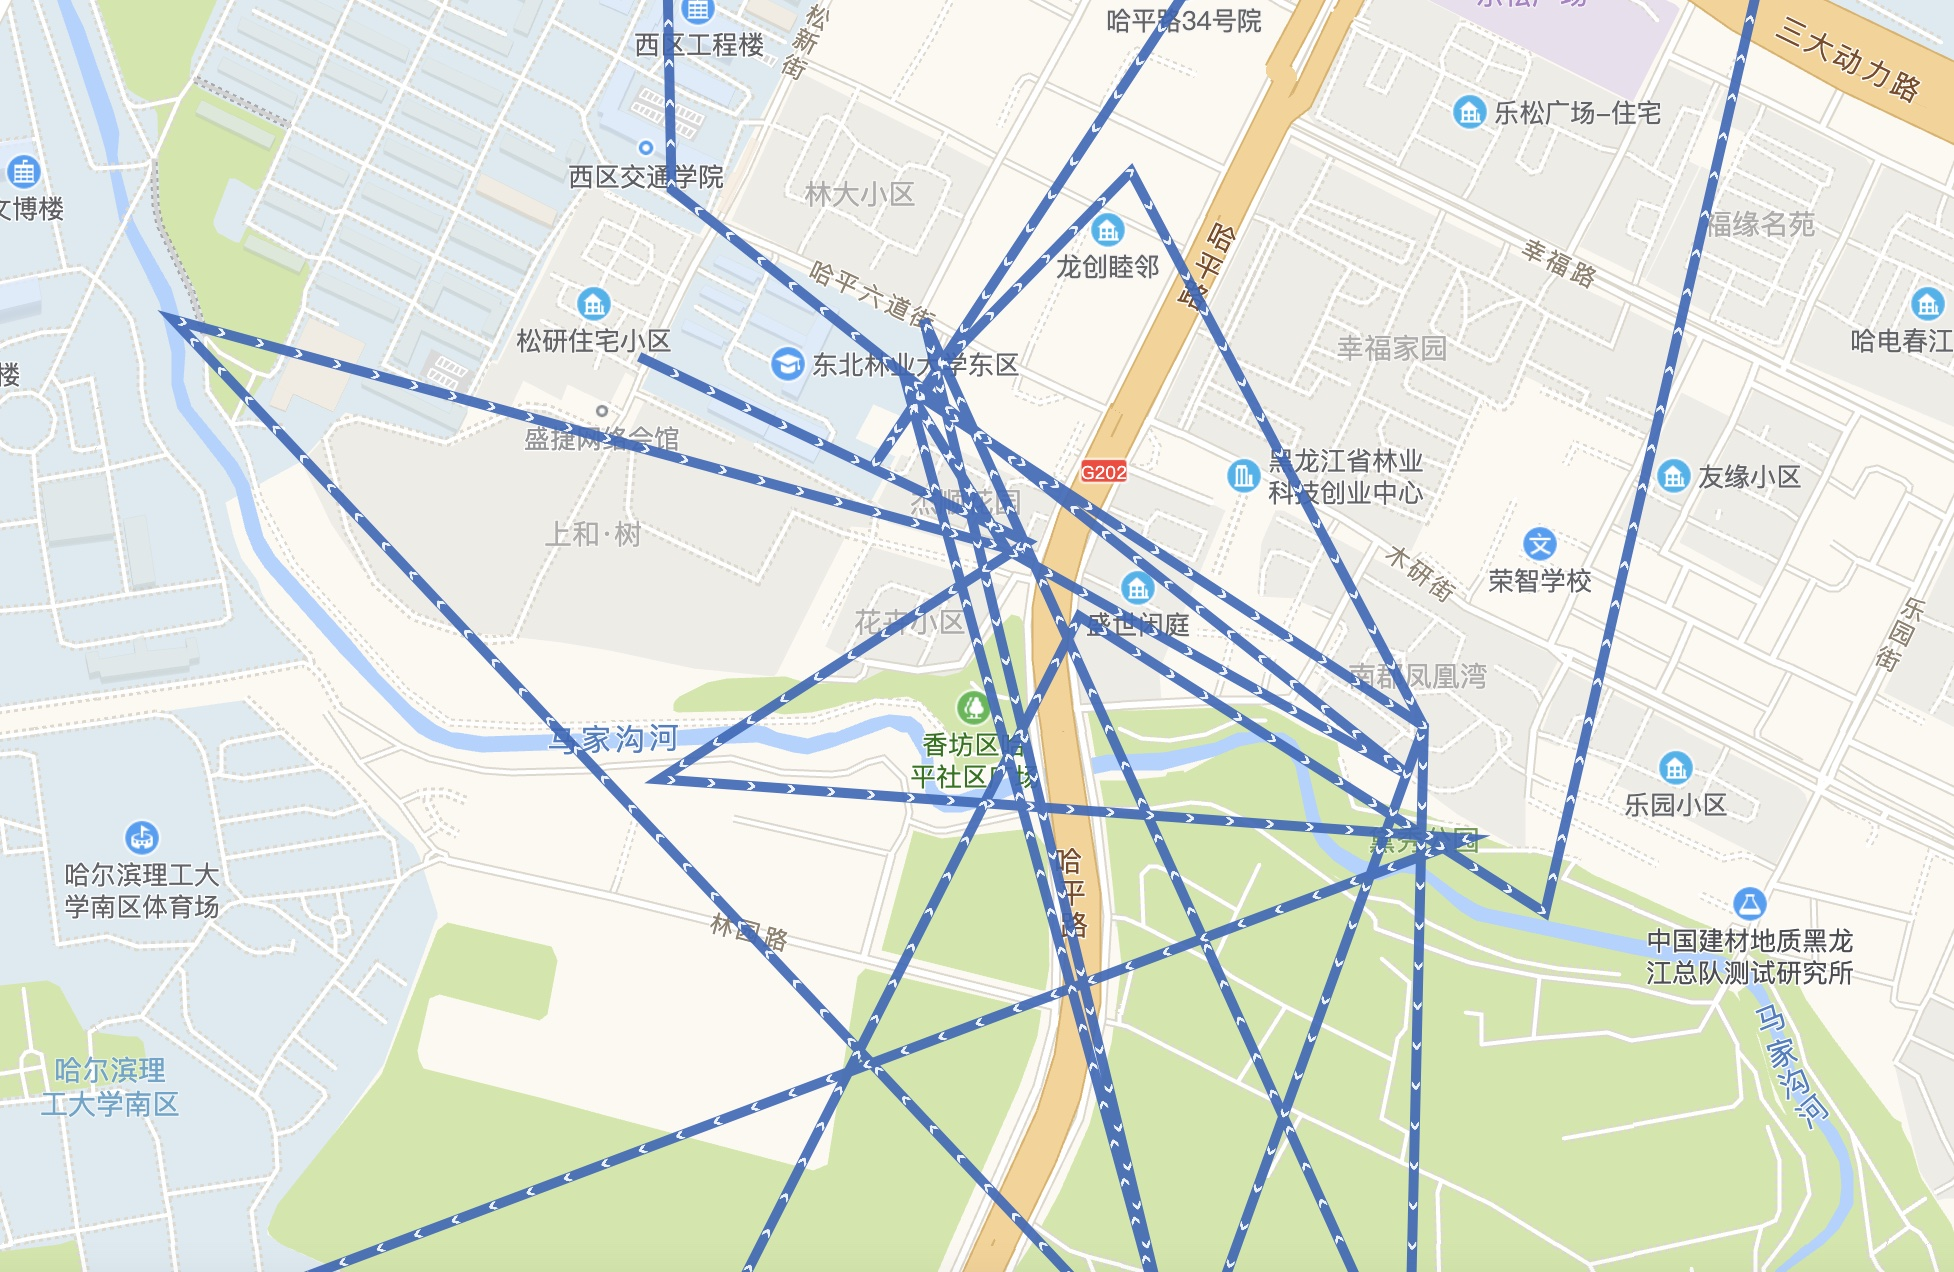
\includegraphics[width = 0.9\textwidth]{track.jpg}
        \caption{基站连接轨迹图}
        \label{fig:track}
    \end{minipage}
    \begin{minipage}[t]{0.49\textwidth}
        \centering
        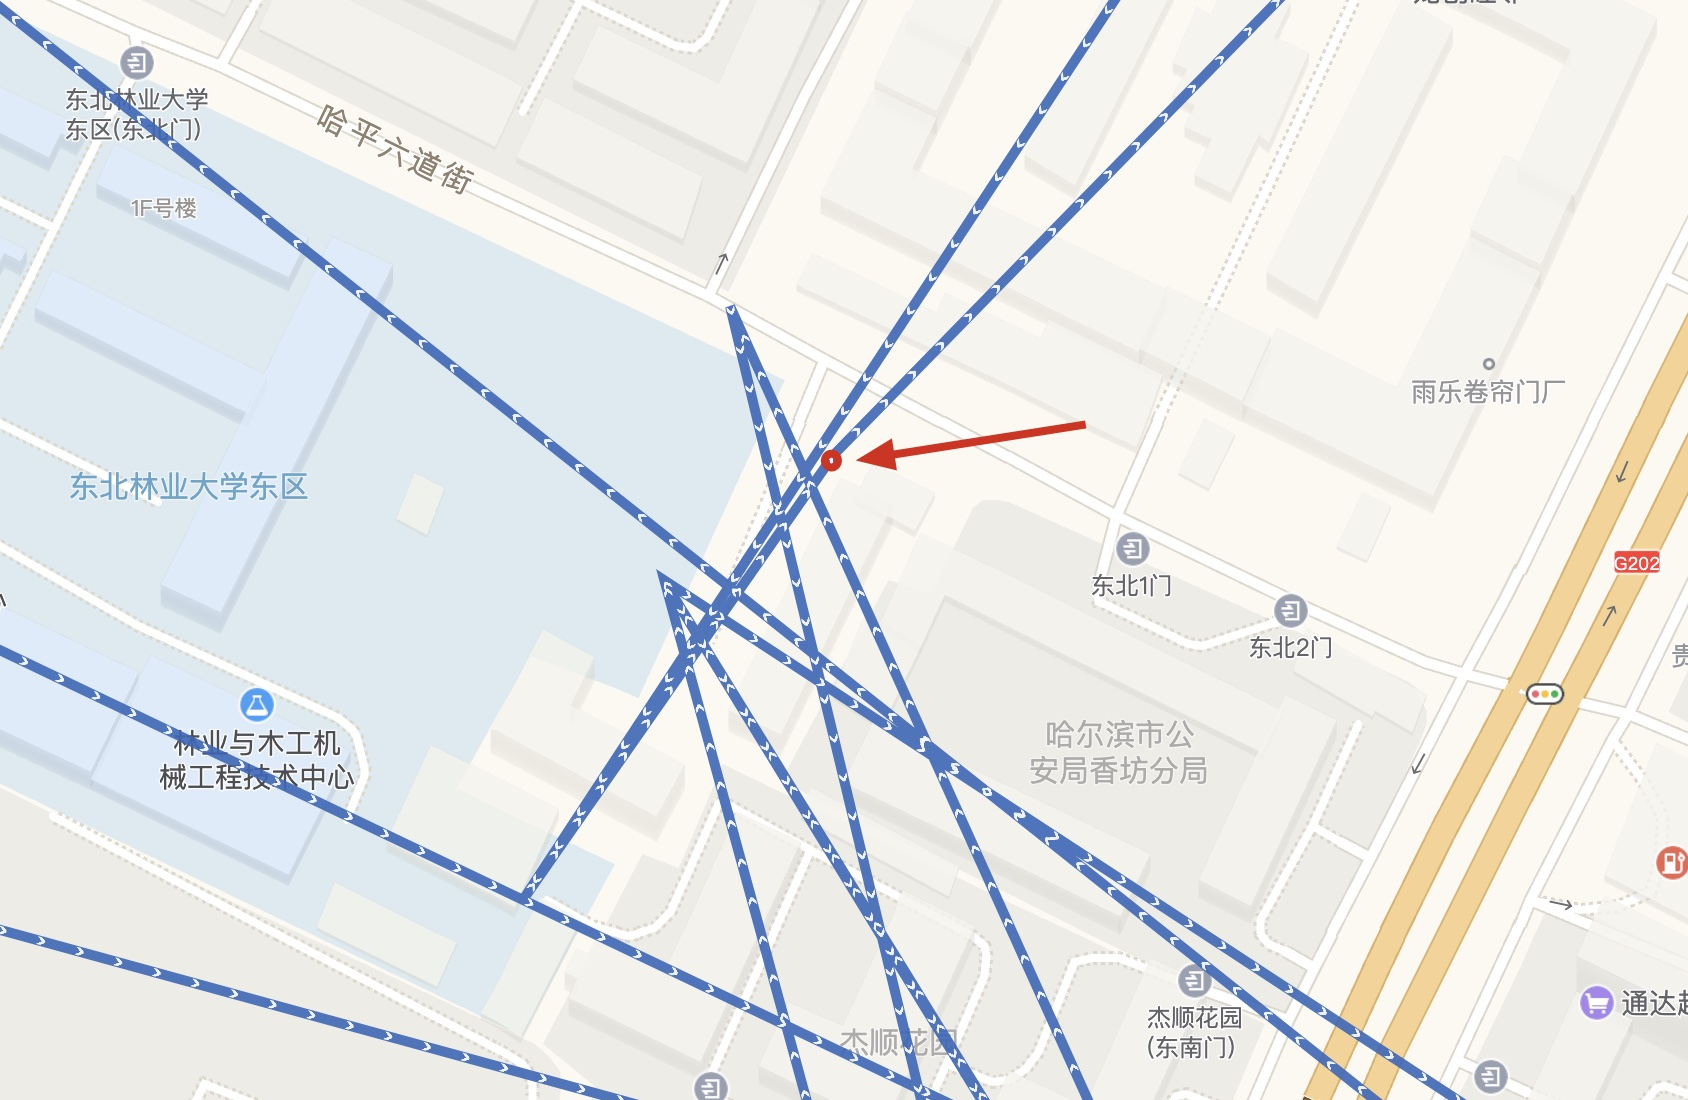
\includegraphics[width = 0.9\textwidth]{stop.jpg}
        \caption{停留地点}
        \label{fig:stop}
    \end{minipage}
\end{figure}

不过由于基站的覆盖面积实在是太大,如图 \ref{fig:cell_con} 中所示,2020 年 1 月 1 日,研究人员本人一天只前往过教化街附近的学生十八公寓、学苑楼、诚意楼,但是却能连接到学校西北部哈尔滨银行附近的一个基站长达 2.1 个小时,以及曲线街(图中未显示,连接次数排名第 5)移动营业厅附近一基站一小时左右。基站的连接轨迹并不能准确的表达用户的真实位置,后面几章将会如何利用基站经纬度坐标推算用户驻留点偏好。

\begin{figure}[ht]
    \centering
    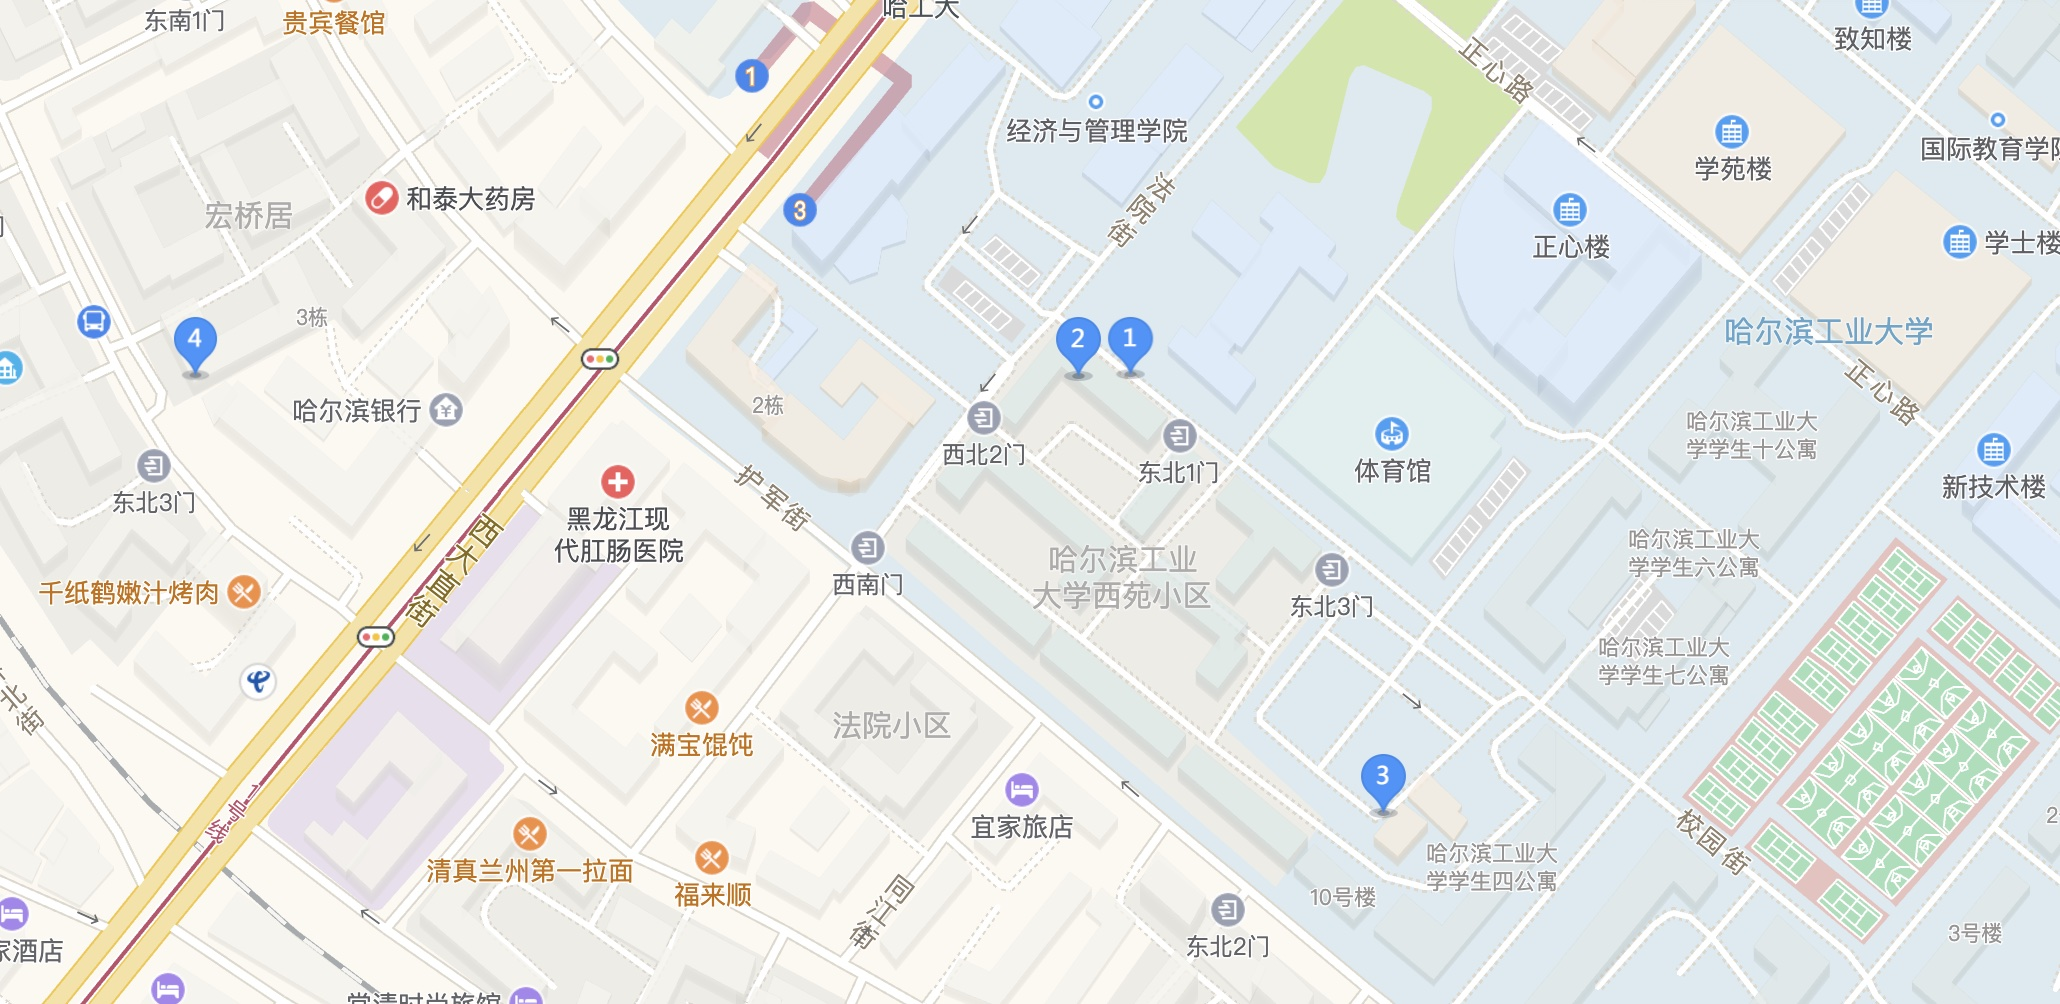
\includegraphics[width = 0.8\textwidth]{cell_con.jpg}
    \caption{连接的最多的基站}
    \label{fig:cell_con}
\end{figure}

\section{哈尔滨市 POI 兴趣点爬取、处理和描述分析}

首先从高德地图上爬取哈尔滨市所有的 POI 兴趣点的相关信息,包括 POI 兴趣点的序号、名称、类型(如购物中心、餐厅、体育场、学校等)、POI 经纬度信息,数据结构如表 \ref{tab:poi_info} 所示。

\begin{table}[htbp]
    \caption{哈尔滨市 POI 兴趣点数据结构}
    \vspace{0.5em}\centering\wuhao
    \begin{tabular}{ccccc}
        \toprule[1.5pt]
        变量名 & 数据名称 & 数据类型 & 样例 & 备注 \\
        \midrule[1pt]
        id & 兴趣点 id & int & 123 & 兴趣点唯一标识符 \\
        name & 兴趣点名称 & string & 远大购物中心 & 名称描述 \\
        type & 兴趣点类型 & string & 购物中心 & 类型描述 \\
        lon & POI 位置经度 & double & 126.556693 & \\
        lat & POI 位置维度 & double & 45.738066 & \\
        \bottomrule[1.5pt]
    \end{tabular}
    \label{tab:poi_info}
\end{table}

\begin{figure}[htbp]
    \centering
    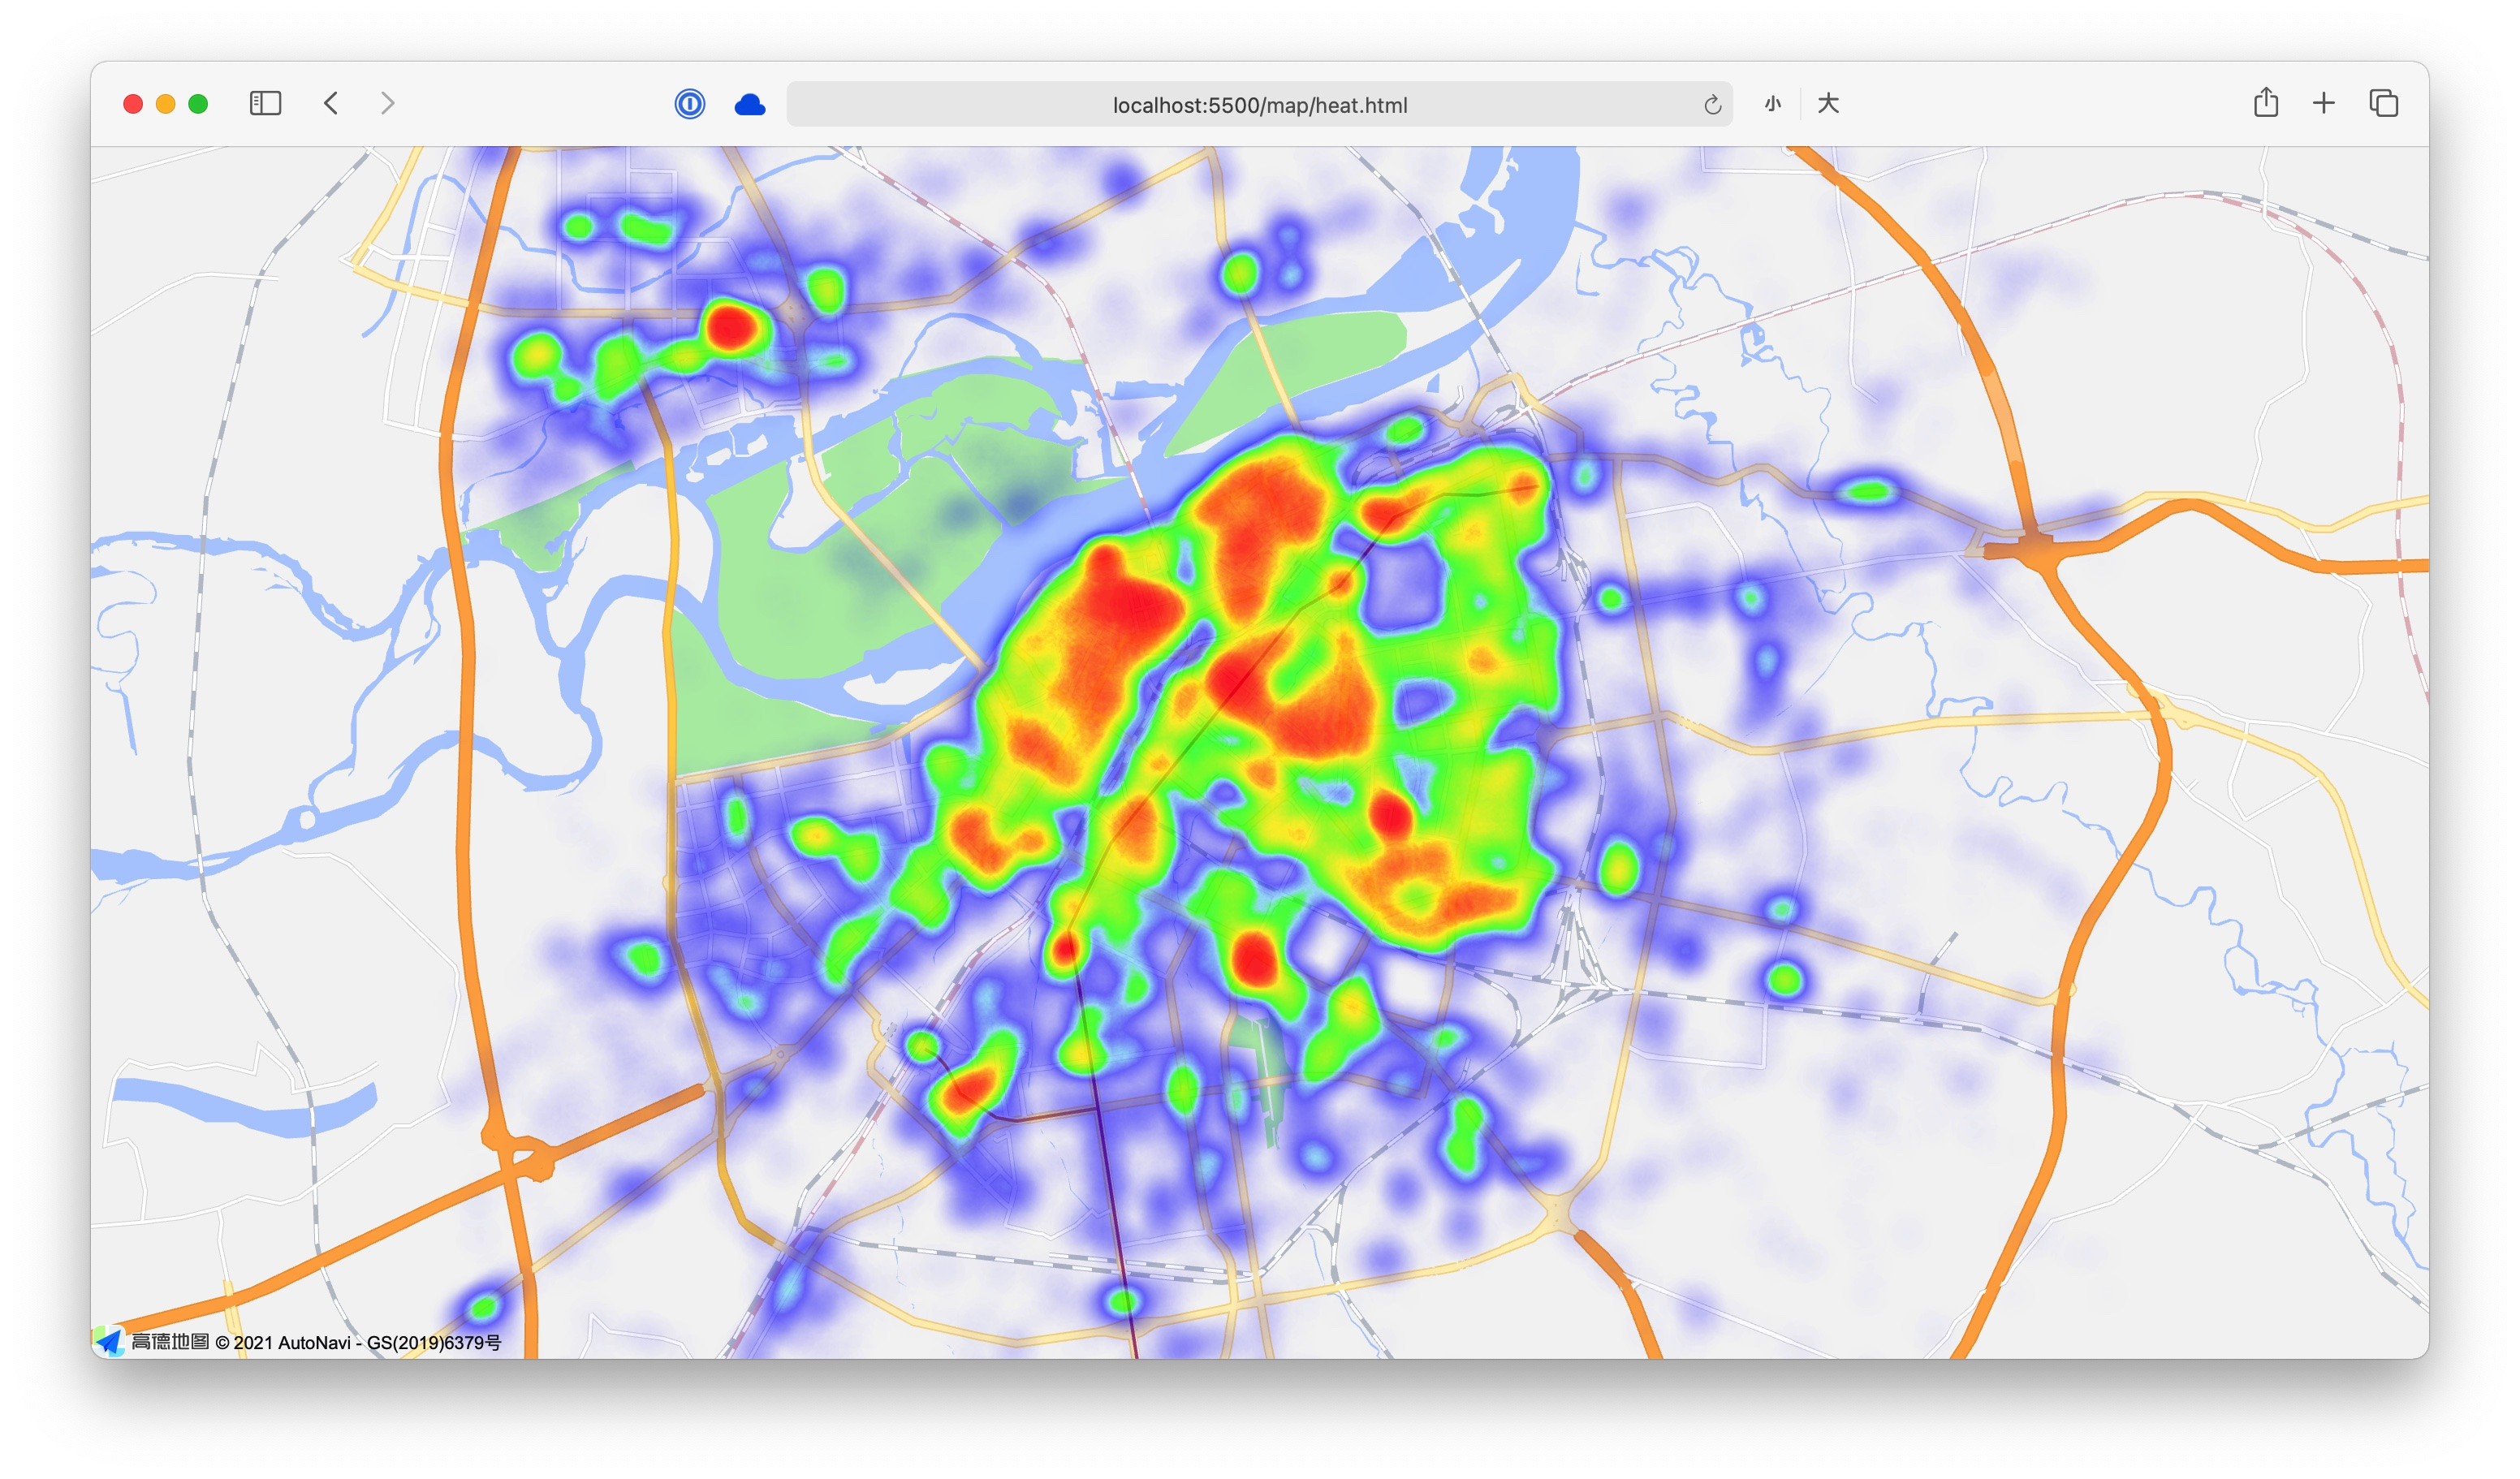
\includegraphics[width = 0.9\textwidth]{poi_gen.jpg}
    \caption{全市 POI 兴趣点分布热力图}
    \label{fig:poi_gen}
\end{figure}

一共 477932 个 POI 兴趣点,每个兴趣点间隔最小小于 1m(经纬度描述相同),最远一千米以上。基站分布如图 \ref{fig:poi_gen} 所示。根据用户基站连接数据统计数据、POI 分布热力图所描述,用户在环城高速以内的活动更为活跃同时用以描述用户移动语义的 POI 兴趣点也更多,所以我们选择哈尔滨市绕城高速以内的市区进行分析,如图 \ref{fig:harbin_raocheng} 所示。

\begin{figure}[htbp]
    \centering
    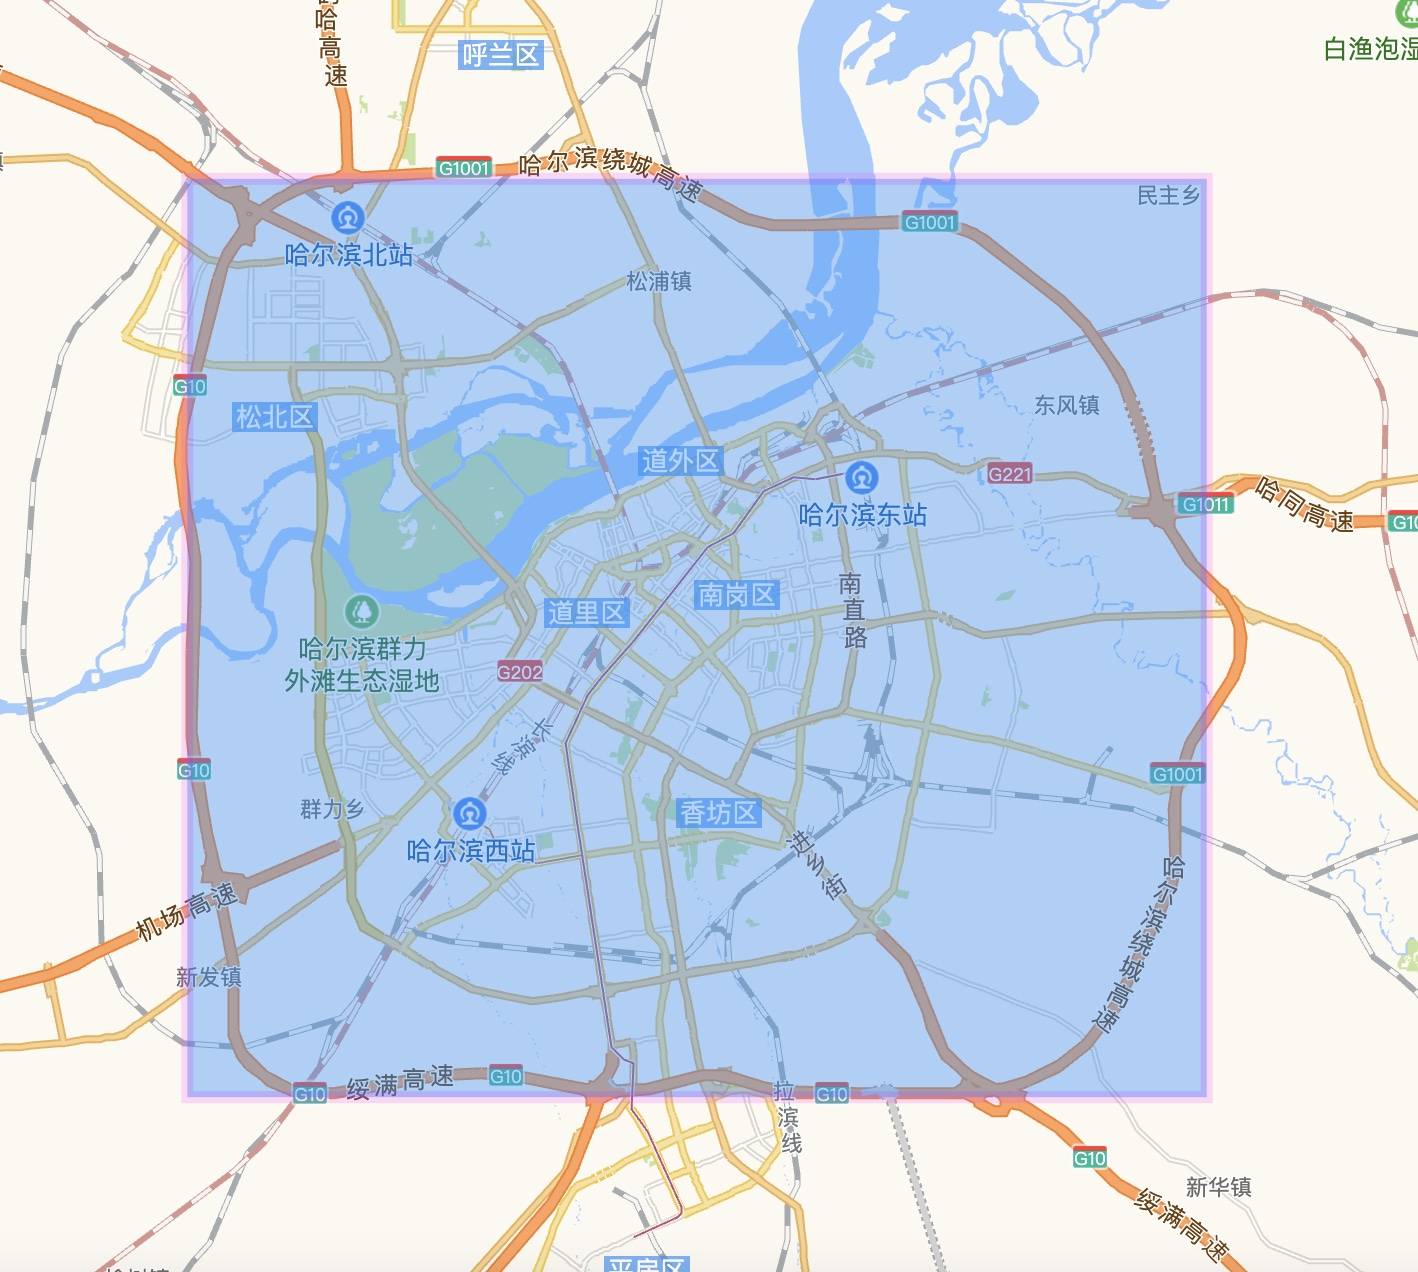
\includegraphics[width = 0.5\textwidth]{district.jpg}
    \caption{哈尔滨市绕城高速范围}
    \label{fig:harbin_raocheng}
\end{figure}

\section{用户手机应用使用流量记录表分析}

\begin{table}[htbp]
    \caption{哈尔滨市用户各个基站的分时流量数据表}
    \vspace{0.5em}\centering\wuhao
    \begin{tabular}{ccccc}
        \toprule[1.5pt]
        变量名 & 数据名称 & 数据类型 & 样例 & 备注 \\
        \midrule[1pt]
        date & 日期 & string & 20200615 & \\
        user\_id & 用户 id & string & 13912345678 & 用户唯一标识符 \\
        app\_id & 手机应用 id & string & C946 & 手机应用唯一标识符 \\
        app\_name & 应用名称 & string & 腾讯视频 & \\
        lon & POI 位置经度 & double & 126.556693 & \\
        lat & POI 位置维度 & double & 45.738066 & \\
        data & 流量数据(单位 B) & int & 578 & 每个小时一个数据,共 8 列 \\
        \bottomrule[1.5pt]
    \end{tabular}
    \label{tab:app_use}
\end{table}

由于 4G 网络在中国的快速铺开,网民飞速增长的同时,移动端应用的使用也越来越频繁,哈尔滨市用户日手机应用流量使用记录数据表可达 600MB,包括记录的日期,用户 id(即手机号码),应用 id(应用商店中应用的唯一标识符),应用名称,基站经纬度,以及从 0 时到 23 时的流量使用数据(单位 Byte),数据结构如表 \ref{tab:app_use} 所示。

爬取手机应用商店中的数据(此处选择华为手机应用商店),经统计,一共 4563 款下载量明显的手机应用,数据维度过多,此处选择使用手机应用的二级类型数据进行降维处理,转为统计用户在某个时间段对某类应用的偏好。爬取的应用数据中包含:如为了和用户应用使用信息表匹配的应用唯一标识符 id,应用一级类型,应用二级类型,下载量,评分等,数据结构如表 \ref{tab:app_info} 所示。

\begin{table}[htbp]
    \caption{手机应用基本信息表}
    \vspace{0.5em}\centering\wuhao
    \begin{tabular}{ccccc}
        \toprule[1.5pt]
        变量名 & 数据名称 & 数据类型 & 样例 & 备注 \\
        \midrule[1pt]
        app\_id & 手机应用 id & string & C946 & 手机应用唯一标识符 \\
        type\_1 & 应用一级类型 & string & 社交软件 & \\
        type\_2 & 应用二级类型 & string & 聊天 & \\
        download & 下载量 & int & 50912769 & 截止到爬取时 \\
        score & 评分 & double & 3.5 & 满分 5 分 \\
        \bottomrule[1.5pt]
    \end{tabular}
    \label{tab:app_info}
\end{table}

\section{用户通话和短信使用记录数据表分析}

为了描述用户的社交地位和偏好,还需要使用用户通话和短信使用记录的相关数据,通话数据包括统计的月份,拨出手机号码,接收手机号码,对端归属地,通话时长,通话次数,通话天数等,数据结构如表 \ref{tab:call_data} 所示。

\begin{table}[htbp]
    \caption{手机应用基本信息表}
    \vspace{0.5em}\centering\wuhao
    \begin{tabular}{ccccc}
        \toprule[1.5pt]
        变量名 & 数据名称 & 数据类型 & 单位 \\
        \midrule[1pt]
        stat\_mon & 统计月份 & string & \\
        serv\_no & 手机号码 & string & \\
        opp\_serv\_no & 对端号码 & string & \\
        opp\_type & 对端类型 & string & \\
        opp\_region\_code & 对端归属地 & string & \\
        call\_dur & 通话时长 & long & 秒 \\
        calling\_dur & 通话时长(主叫) & long & 秒 \\
        called\_dur & 通话时长(被叫) & long & 秒 \\
        call\_cnt & 通话次数 & long & 次 \\
        calling\_cnt & 通话次数(主叫) & long & 次 \\
        called\_cnt & 通话次数(被叫) & long & 次 \\
        busy\_call\_cnt & 忙时通话次数 & long & 次 \\
        idle\_call\_cnt & 闲时通话次数 & long & 次 \\
        busy\_dur & 忙时通话时长 & long & 分钟 \\
        idle\_dur & 闲时通话时长 & long & 分钟 \\
        weekday\_sum\_call\_cnt & 工作日通话次数 & long & 次 \\
        weekday\_work\_sum\_call\_cnt & 工作日上班时间通话次数 & long & 次 \\
        weekday\_offwork\_sum\_call\_cnt & 工作日非上班时间通话次数 & long & 次 \\
        weekend\_sum\_call\_cnt & 周末通话次数 & long & 次 \\
        weekday\_sum\_call\_dur & 工作日通话时长 & long & 分钟 \\
        weekend\_sum\_call\_dur & 周末通话时长 & long & 分钟 \\
        call\_days & 通话天数 & long & 天 \\
        first\_call\_date & 末次通话时间 & string & \\
        last\_call\_date & 首次通话时间 & string & \\
        \bottomrule[1.5pt]
    \end{tabular}
    \label{tab:call_data}
\end{table}

同理,用户点对点短信记录信息表中包含统计日期、用户类型、发送方号码、发送方归属区号、接收方号码、接收方归属区号、短信条数等信息,数据结构如表 \ref{tab:msg_data} 所示。

\begin{table}[htbp]
    \caption{手机应用基本信息表}
    \vspace{0.5em}\centering\wuhao
    \begin{tabular}{ccccc}
        \toprule[1.5pt]
        变量名 & 数据名称 & 数据类型 \\
        \midrule[1pt]
        stats\_mon & 统计月份 & string \\
        user\_type & 用户类型 & string \\
        send\_serv\_no & 发送方手机号码 & string \\
        home\_city\_code & 发送方归属区号 & string \\
        reci\_serv\_no & 接收方手机号码 & string \\
        opp\_city\_code & 接收方归属区号 & string \\
        gms\_count & 短信条数 & long \\
        \bottomrule[1.5pt]
    \end{tabular}
    \label{tab:msg_data}
\end{table}

\section{本章小结}

本章通过对原始数据的统计性描述和分析,首先确定了可用的数据库和能用以分析用户画像的数据的结构,统计数据中可能有误和缺失的信息,做好标记用以支持之后的正式处理中采用剔除或默认值的办法替换原值;同时统计数量大小和有效数据范围,如每日信息数量、统计区域范围(哈尔滨市绕城高速)等,为后续小样本的计算模型测试提供理论基础;

\chapter{哈尔滨市城区 POI 兴趣点数据获分析和栅格化街区聚类分析}

\section{哈尔滨市城区 POI 兴趣点数据具体分析}

为了能够描述用户的移动语义(即用户前往目的地的原因),同时由于基站的覆盖面积过于宽广,并不能直接将基站的位置认为是用户的目的位置,文献 \cite{phithakkitnukoon_activity-aware_2010}\cite{dashdorj_semantic_2018} 中 Phithakkinukoon 和 Dashjor 指出,用户的移动语义是由某一个范围内的兴趣点的分布情况决定的,如果得知了该区块中各类型兴趣点的分布,那么我们就能大致推算前往该区域的用户的目的。

如图 \ref{fig:hit_poi},为哈尔滨工业大学一校区周边 POI 兴趣点分布地图,若一个区域中分布着教学楼、公寓、食堂、超市等兴趣点,

\begin{figure}[htbp]
    \centering
    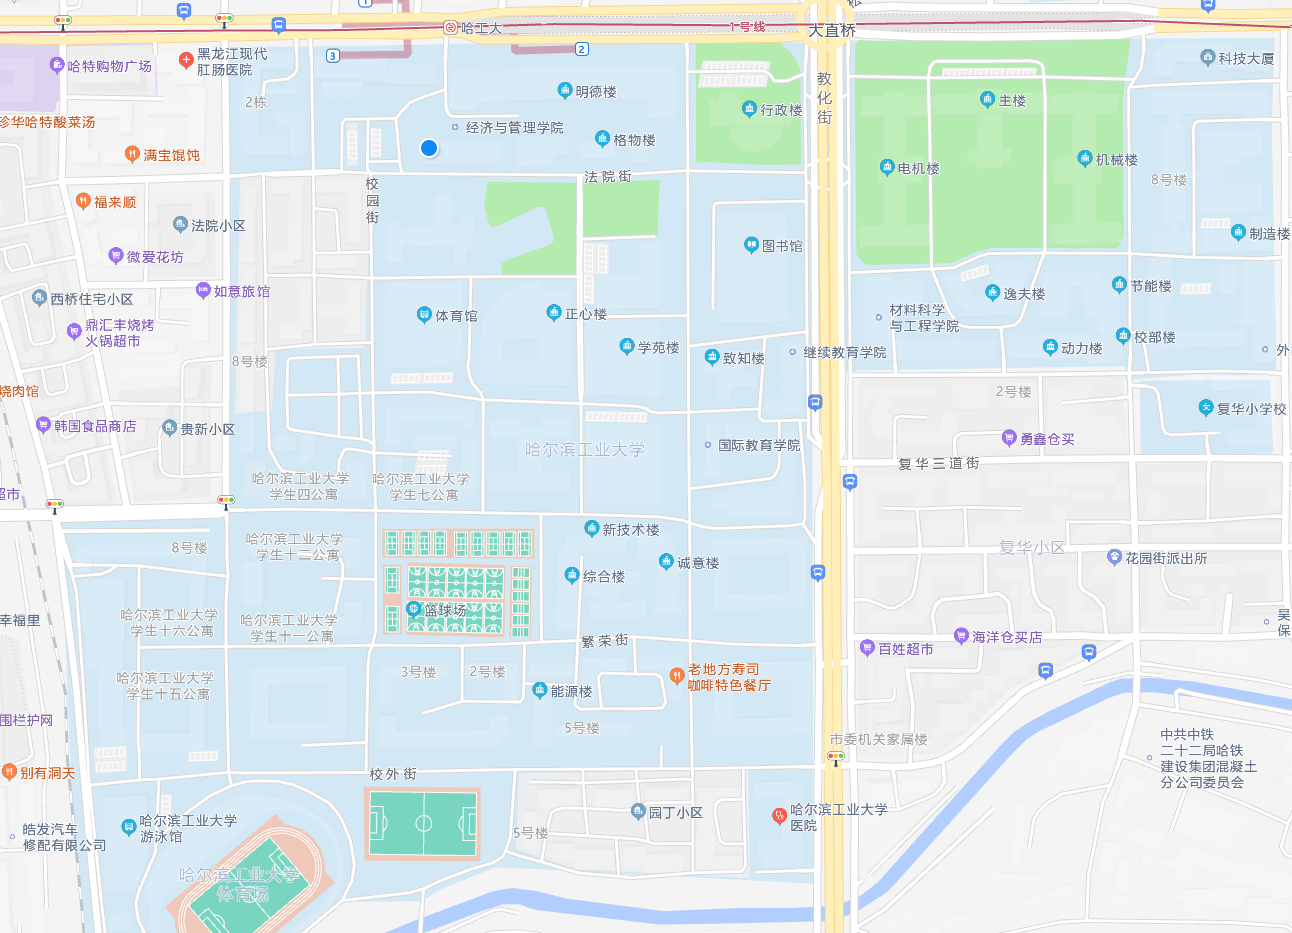
\includegraphics[width = 0.9\textwidth]{hit_poi.png}
    \caption{哈尔滨工业大学一校区周边 POI 兴趣点分布图}
    \label{fig:hit_poi}
\end{figure}

\section{基于路网和栅格化的功能区聚类分析模型对比}

\section{功能区的栅格化参数的分析和对比}

\section{本章小结}

\chapter{大数据领域下聚类方法的对比和在哈尔滨城市功能区的聚类结果分析}

\section{DBSCAN 聚类算法概述和分析}

\section{K-Means 聚类算法概述}

K-Means 算法的思想非常简单,对于样本集,按照距离划分为若干个簇,让簇内距离最小化,簇间距离最大化。如果有集合 $G$,假设划分的簇为\\ $(U_1, U_2, \dots, U_m)$,则我们的目标则是最小化误差 $E$:

$$
E = \sum_{i=1}^{m}\sum_{x \in U_{i}} ||x - \mu_{i}||^{2}_{2}
$$

其中,$\mu_{i}$ 是每个簇的质心,通常是一个均值向量。传统的算法通常是随机选择 $k$ 质心(即要分成多少类),经常会根据先验经验做一个 $k$ 值选择,对于每一次迭代,求每个点到每个质心的距离,最小距离则为改簇,重复迭代,直到质心没有变化。

\section{K-Means 初始质心选择优化 K-Means++ 算法}

在最基础的 K-Means 聚类中,最初的质心的选择通常是随机选择,而在 K-Means++ 中,则是优化最初的质心选择,优化策略也比较简单,方法如下:

\begin{enumerate}
    \item 随机选择一个点作为第一个质心 $\mu_{1}$;
    \item 对于寻找第 $i$ 个质心,则计算数据集中没有作为质心的点,分别到前 $i - 1$ 个质心的最小距离 $D_{j} = \min(Distance(j, i))$;
    \item 有概率的选择第 $i$ 个质心,原则是 $D_{j}$ 越大的点作为第 $i$ 个质心的概率越大;
    \item 重复,选出 $k$ 个质心;
\end{enumerate}

但是 K-Means 的优化只能优化迭代的次数,而 K-Means 的算法复杂度是 $O(MNKD)$,$N$ 为样本数量,$K$ 为聚类个数,$D$ 为数据维度,$M$ 与数据集本身的分布情况和中心点有关 \emph{此处有引用},K-Means++ 的优化对于本研究 4 百万的原数样本数量来说,并不是特别的高效。

\section{大样本优化 Mini Batch K-Means 算法}

在上上节所述的 K-Means 的传统算法中,每次迭代都需要计算数据集中每个节点到质心的距离,当数据量达到 10 万以上时,即使加上诸如 elkan K-Means 优化\emph{此处有引用} 也无法应付。此时,就要用到 Mini Batch K-Means 算法。

如同字面意思,Mini Batch,原理十分简单,从数据集中随机抽取一部分样本,做普通的 K-Means 聚类,得到的质心就被认定为最终的质心。由于 $N$ 缩小的很快,导致算法每次跌打的速度大大加快,当然,精度也会降低,不过经过证明 \emph{此处有引用},仍然在我们的可接受范围内,而且通常会进行多次 Mini Batch K-Means 聚类,选择其中最优的聚类结果。

如图  的一次 K-Means 与 Mini Batch K-Means 对比,二者的运行时间相差两倍多,但最终的结果差异确非常小,图中第三张(Difference)的粉色错误点。

\section{哈尔滨市功能区聚类结果分析和展示}

\section{本章小结}

\chapter{大数据系统不同计算框架的分析与对比}

\chapter{基于手机信令数据的用户驻留点、手机应用偏好以及社交地位分析}

\chapter{基于驻留点、应用偏好和社交地位分析结果的用户职住特征分析}

% Local Variables:
% TeX-master: "../main"
% TeX-engine: xetex
% End:

\backmatter
% !Mode:: "TeX:UTF-8" 
\begin{conclusions}

学位论文的结论作为论文正文的最后一章单独排写,但不加章标题序号。

结论应是作者在学位论文研究过程中所取得的创新性成果的概要总结,不能与摘要混为一谈。博士学位论文结论应包括论文的主要结果、创新点、展望三部分,在结论中应概括论文的核心观点,明确、客观地指出本研究内容的创新性成果(含新见解、新观点、方法创新、技术创新、理论创新),并指出今后进一步在本研究方向进行研究工作的展望与设想。对所取得的创新性成果应注意从定性和定量两方面给出科学、准确的评价,分(1)、(2)、(3)…条列出,宜用“提出了”、“建立了”等词叙述。

\end{conclusions}
   % 结论
\bibliographystyle{hithesis} %如果没有参考文献时候
\bibliography{reference}
%%%%%%%%%%%%%%%%%%%%%%%%%%%%%%%%%%%%%%%%%%%%%%%%%%%%%%%%%%%%%%%%%%%%%%%%%%%%%%%% 
%-- 注意:以下本硕博、博后书序不一致 --%
%%%%%%%%%%%%%%%%%%%%%%%%%%%%%%%%%%%%%%%%%%%%%%%%%%%%%%%%%%%%%%%%%%%%%%%%%%%%%%%% 
% 硕博书序
%%%%%%%%%%%%%%%%%%%%%%%%%%%%%%%%%%%%%%%%%%%%%%%%%%%%%%%%%%%%%%%%%%%%%%%%%%%%%%%% 
% \begin{appendix}%附录
% % -*-coding: utf-8 -*-
%%%%%%%%%%%%%%%%%%%%%%%%%%%%%%%%%%%%%%%%%%%%%%%%%%%%%%%%%
\chapter{带章节的附录}[Full Appendix]%
完整的附录内容,包含章节,公式,图表等

%%%%%%%%%%%%%%%%%%%%%%%%%%%%%%%%%%%%%%%%%%%%%%%%%%%%%%%%%
\section{附录节的内容}[Section in Appendix]
这是附录的节的内容

附录中图的示例:
\begin{figure}[htbp]
\centering
\includegraphics[width = 0.4\textwidth]{golfer}
%\bicaption[golfer5]{}{\xiaosi[0]打高尔夫球的人}{Fig.$\!$}{The person playing golf}\vspace{-1em}
\caption{\xiaosi[0]打高尔夫球的人}
\end{figure}

附录中公式的示例:
\begin{align}
a & = b \times c \\
E & = m c^2
\label{eq}
\end{align}

\chapter{这个星球上最好的免费Linux软件列表}[List of the Best Linux Software in our Planet]
\section{系统}

\href{http://fvwm.org/}{FVWM 自从上世纪诞生以来,此星球最强大的窗口管理器。}
推荐基于FVWM的桌面设计hifvwm:\href{https://github.com/dustincys/hifvwm}{https://github.com/dustincys/hifvwm}。

\subsection{hifvwm的优点}

\begin{enumerate}
	\item 即使打开上百个窗口也不会“蒙圈”。计算机性能越来越强大,窗口任务的管理必须要升级到打怪兽级别。
	\item 自动同步Bing搜索主页的壁纸。每次电脑开机,午夜零点自动更新,用户
		也可以手动更新,从此审美再也不疲劳。
	\item 切换窗口自动聚焦到最上面的窗口。使用键盘快捷键切换窗口时候,减少
		操作过程,自动聚焦到目标窗口。这一特性是虚拟窗口必须的人性化设
		计。
	\item 类似window右下角的功能的最小化窗口来显示桌面的功能此处类似
		win7/win10,实现在一个桌面之内操作多个任务。
	\item 任务栏结合标题栏。采用任务栏和标题栏结合,节省空间。
	\item 同类窗口切换。可以在同类窗口之内类似alt-tab的方式切换。
	\item ……
\end{enumerate}

\section{其他}

\href{https://github.com/goldendict/goldendict}{goldendict 星球最强大的桌面字典。}

\href{https://github.com/yarrick/iodine}{iodine,“HIT-WLAN + 锐捷”时代的福音。}

\href{http://www.aircrack-ng.org/}{aircrack,Wifi“安全性评估”工具。}

\href{https://www.ledger-cli.org/}{ledger,前“金融区块链”时代最好的复式记账系统。}

\href{https://orgmode.org/}{orgmode,最强大的笔记系统,从来没有之一。}

\href{https://www.jianguoyun.com/}{坚果云,国内一款支持WebDav的云盘系统,国内真正的云盘没有之一。}

\href{http://www.mutt.org/}{mutt, ``All mail clients suck. This one just sucks less.''}

\section{vim}
实现中英文每一句一行,以及实现每一句折叠断行的简单正则式,tex源码更加乖乖。
\begin{lstlisting}
vnoremap <leader>fae J:s/[.!?]\zs\s\+/\="\r".matchstr(getline('.'), '^\s*')/g<CR>
vnoremap <leader>fac J:s/[。!?]/\=submatch(0)."\n".matchstr(getline('.'), '^\s*')/g<CR>
vnoremap <leader>fle :!fmt -80 -s<CR>
\end{lstlisting}

% \end{appendix}
% % !Mode:: "TeX:UTF-8" 
\begin{publication}
\noindent\textbf{发表的相关论文}
\begin{publist}
\item	XXX,XXX. Static Oxidation Model of Al-Mg/C Dissipation Thermal Protection Materials[J]. Rare Metal Materials and Engineering, 2010, 39(Suppl. 1): 520-524.(SCI~收录,IDS号为~669JS,IF=0.16)
\item XXX,XXX. 精密超声振动切削单晶铜的计算机仿真研究[J]. 系统仿真学报,2007,19(4):738-741,753.(EI~收录号:20071310514841)
\item XXX,XXX. 局部多孔质气体静压轴向轴承静态特性的数值求解[J]. 摩擦学学报,2007(1):68-72.(EI~收录号:20071510544816)
\item XXX,XXX. 硬脆光学晶体材料超精密切削理论研究综述[J]. 机械工程学报,2003,39(8):15-22.(EI~收录号:2004088028875)
\item XXX,XXX. 基于遗传算法的超精密切削加工表面粗糙度预测模型的参数辨识以及切削参数优化[J]. 机械工程学报,2005,41(11):158-162.(EI~收录号:2006039650087)
\item XXX,XXX. Discrete Sliding Mode Cintrok with Fuzzy Adaptive Reaching Law on 6-PEES Parallel Robot[C]. Intelligent System Design and Applications, Jinan, 2006: 649-652.(EI~收录号:20073210746529)
\end{publist}

\noindent\textbf{(二)申请及已获得的专利(无专利时此项不必列出)}
\begin{publist}
\item XXX,XXX. 一种温热外敷药制备方案:中国,88105607.3[P]. 1989-07-26.
\end{publist}

\noindent\textbf{(三)参与的科研项目及获奖情况}
\begin{publist}
\item	XXX,XXX. XX~气体静压轴承技术研究, XX~省自然科学基金项目.课题编号:XXXX.
\item XXX,XXX. XX~静载下预应力混凝土房屋结构设计统一理论. 黑江省科学技术二等奖, 2007.
\end{publist}
%\vfill
%\hangafter=1\hangindent=2em\noindent
%\setlength{\parindent}{2em}
\end{publication}
    % 所发文章
% \begin{ceindex}
  %如果想要手动加索引,注释掉以下这一样,用wordlist环境
\printsubindex*
\end{ceindex}
    % 索引, 根据自己的情况添加或者不添加,选择自动添加或者手工添加。
% \authorization %授权
% %\authorization[scan.pdf] %添加扫描页的命令,与上互斥
% % !Mode:: "TeX:UTF-8"
\begin{acknowledgements}
衷心感谢导师~XXX~教授对本人的精心指导。他的言传身教将使我终生受益。

……

感谢哈工大\LaTeX\ 论文模板\hithesis\ !

\end{acknowledgements}
 %致谢
% % !Mode:: "TeX:UTF-8" 

\begin{resume}
XXXX~年~XX~月~XX~日出生于~XXXX。

XXXX~年~XX~月考入~XX~大学~XX~院(系)XX~专业,XXXX~年~XX~月本科毕业并获得~XX~学学士学位。

XXXX~年~XX~月------XXXX~年~XX~月在~XX~大学~XX~院(系)XX~学科学习并获得~XX~学硕士学位。

XXXX~年~XX~月------XXXX~年~XX~月在~XX~大学~XX~院(系)XX~学科学习并获得~XX~学博士学位。

获奖情况:如获三好学生、优秀团干部、X~奖学金等(不含科研学术获奖)。

工作经历:

\textbf{( 除全日制硕士生以外,其余学生均应增列此项。个人简历一般应包含教育经历和工作经历。)}
\end{resume}
          % 博士学位论文有个人简介
%%%%%%%%%%%%%%%%%%%%%%%%%%%%%%%%%%%%%%%%%%%%%%%%%%%%%%%%%%%%%%%%%%%%%%%%%%%%%%%% 
% 本科书序为:
%%%%%%%%%%%%%%%%%%%%%%%%%%%%%%%%%%%%%%%%%%%%%%%%%%%%%%%%%%%%%%%%%%%%%%%%%%%%%%%% 
\authorization %授权
% \authorization[scan.pdf] %添加扫描页的命令,与上互斥
% !Mode:: "TeX:UTF-8"
\begin{acknowledgements}
衷心感谢导师~XXX~教授对本人的精心指导。他的言传身教将使我终生受益。

……

感谢哈工大\LaTeX\ 论文模板\hithesis\ !

\end{acknowledgements}
 %致谢
\begin{appendix}%附录
    \chapter{外文资料原文}
\label{cha:engorg}

\title{The title of the English paper}

\textbf{Abstract:} As one of the most widely used techniques in operations
research, \emph{ mathematical programming} is defined as a means of maximizing a
quantity known as \emph{bjective function}, subject to a set of constraints
represented by equations and inequalities. Some known subtopics of mathematical
programming are linear programming, nonlinear programming, multiobjective
programming, goal programming, dynamic programming, and multilevel
programming$^{[1]}$.

It is impossible to cover in a single chapter every concept of mathematical
programming. This chapter introduces only the basic concepts and techniques of
mathematical programming such that readers gain an understanding of them
throughout the book$^{[2,3]}$.


\section{Single-Objective Programming}
The general form of single-objective programming (SOP) is written
as follows,
\begin{equation}\tag*{(123)} % 如果附录中的公式不想让它出现在公式索引中,那就请
                             % 用 \tag*{xxxx}
\left\{\begin{array}{l}
\max \,\,f(x)\\[0.1 cm]
\mbox{subject to:} \\ [0.1 cm]
\qquad g_j(x)\le 0,\quad j=1,2,\cdots,p
\end{array}\right.
\end{equation}
which maximizes a real-valued function $f$ of
$x=(x_1,x_2,\cdots,x_n)$ subject to a set of constraints.

\newtheorem{mpdef}{Definition}[chapter]
\begin{mpdef}
In SOP, we call $x$ a decision vector, and
$x_1,x_2,\cdots,x_n$ decision variables. The function
$f$ is called the objective function. The set
\begin{equation}\tag*{(456)} % 这里同理,其它不再一一指定。
S=\left\{x\in\Re^n\bigm|g_j(x)\le 0,\,j=1,2,\cdots,p\right\}
\end{equation}
is called the feasible set. An element $x$ in $S$ is called a
feasible solution.
\end{mpdef}

\newtheorem{mpdefop}[mpdef]{Definition}
\begin{mpdefop}
A feasible solution $x^*$ is called the optimal
solution of SOP if and only if
\begin{equation}
f(x^*)\ge f(x)
\end{equation}
for any feasible solution $x$.
\end{mpdefop}

One of the outstanding contributions to mathematical programming was known as
the Kuhn-Tucker conditions\ref{eq:ktc}. In order to introduce them, let us give
some definitions. An inequality constraint $g_j(x)\le 0$ is said to be active at
a point $x^*$ if $g_j(x^*)=0$. A point $x^*$ satisfying $g_j(x^*)\le 0$ is said
to be regular if the gradient vectors $\nabla g_j(x)$ of all active constraints
are linearly independent.

Let $x^*$ be a regular point of the constraints of SOP and assume that all the
functions $f(x)$ and $g_j(x),j=1,2,\cdots,p$ are differentiable. If $x^*$ is a
local optimal solution, then there exist Lagrange multipliers
$\lambda_j,j=1,2,\cdots,p$ such that the following Kuhn-Tucker conditions hold,
\begin{equation}
\label{eq:ktc}
\left\{\begin{array}{l}
    \nabla f(x^*)-\sum\limits_{j=1}^p\lambda_j\nabla g_j(x^*)=0\\[0.3cm]
    \lambda_jg_j(x^*)=0,\quad j=1,2,\cdots,p\\[0.2cm]
    \lambda_j\ge 0,\quad j=1,2,\cdots,p.
\end{array}\right.
\end{equation}
If all the functions $f(x)$ and $g_j(x),j=1,2,\cdots,p$ are convex and
differentiable, and the point $x^*$ satisfies the Kuhn-Tucker conditions
(\ref{eq:ktc}), then it has been proved that the point $x^*$ is a global optimal
solution of SOP.

\subsection{Linear Programming}
\label{sec:lp}

If the functions $f(x),g_j(x),j=1,2,\cdots,p$ are all linear, then SOP is called
a {\em linear programming}.

The feasible set of linear is always convex. A point $x$ is called an extreme
point of convex set $S$ if $x\in S$ and $x$ cannot be expressed as a convex
combination of two points in $S$. It has been shown that the optimal solution to
linear programming corresponds to an extreme point of its feasible set provided
that the feasible set $S$ is bounded. This fact is the basis of the {\em simplex
  algorithm} which was developed by Dantzig as a very efficient method for
solving linear programming.
\begin{table}[ht]
\centering
  \centering
  \caption*{Table~1\hskip1em This is an example for manually numbered table, which
    would not appear in the list of tables}
  \label{tab:badtabular2}
  \begin{tabular}[c]{|m{1.5cm}|c|c|c|c|c|c|}\hline
    \multicolumn{2}{|c|}{Network Topology} & \# of nodes &
    \multicolumn{3}{c|}{\# of clients} & Server \\\hline
    GT-ITM & Waxman Transit-Stub & 600 &
    \multirow{2}{2em}{2\%}&
    \multirow{2}{2em}{10\%}&
    \multirow{2}{2em}{50\%}&
    \multirow{2}{1.2in}{Max. Connectivity}\\\cline{1-3}
    \multicolumn{2}{|c|}{Inet-2.1} & 6000 & & & &\\\hline
    & \multicolumn{2}{c|}{ABCDEF} &\multicolumn{4}{c|}{} \\\hline
\end{tabular}
\end{table}

Roughly speaking, the simplex algorithm examines only the extreme points of the
feasible set, rather than all feasible points. At first, the simplex algorithm
selects an extreme point as the initial point. The successive extreme point is
selected so as to improve the objective function value. The procedure is
repeated until no improvement in objective function value can be made. The last
extreme point is the optimal solution.

\subsection{Nonlinear Programming}

If at least one of the functions $f(x),g_j(x),j=1,2,\cdots,p$ is nonlinear, then
SOP is called a {\em nonlinear programming}.

A large number of classical optimization methods have been developed to treat
special-structural nonlinear programming based on the mathematical theory
concerned with analyzing the structure of problems.

Now we consider a nonlinear programming which is confronted solely with
maximizing a real-valued function with domain $\Re^n$.  Whether derivatives are
available or not, the usual strategy is first to select a point in $\Re^n$ which
is thought to be the most likely place where the maximum exists. If there is no
information available on which to base such a selection, a point is chosen at
random. From this first point an attempt is made to construct a sequence of
points, each of which yields an improved objective function value over its
predecessor. The next point to be added to the sequence is chosen by analyzing
the behavior of the function at the previous points. This construction continues
until some termination criterion is met. Methods based upon this strategy are
called {\em ascent methods}, which can be classified as {\em direct methods},
{\em gradient methods}, and {\em Hessian methods} according to the information
about the behavior of objective function $f$. Direct methods require only that
the function can be evaluated at each point. Gradient methods require the
evaluation of first derivatives of $f$. Hessian methods require the evaluation
of second derivatives. In fact, there is no superior method for all
problems. The efficiency of a method is very much dependent upon the objective
function.

\subsection{Integer Programming}

{\em Integer programming} is a special mathematical programming in which all of
the variables are assumed to be only integer values. When there are not only
integer variables but also conventional continuous variables, we call it {\em
  mixed integer programming}. If all the variables are assumed either 0 or 1,
then the problem is termed a {\em zero-one programming}. Although integer
programming can be solved by an {\em exhaustive enumeration} theoretically, it
is impractical to solve realistically sized integer programming problems. The
most successful algorithm so far found to solve integer programming is called
the {\em branch-and-bound enumeration} developed by Balas (1965) and Dakin
(1965). The other technique to integer programming is the {\em cutting plane
  method} developed by Gomory (1959).

\hfill\textit{Uncertain Programming\/}\quad(\textsl{BaoDing Liu, 2006.2})

\section*{References}
\noindent{\itshape NOTE: These references are only for demonstration. They are
  not real citations in the original text.}

\begin{translationbib}
\item Donald E. Knuth. The \TeX book. Addison-Wesley, 1984. ISBN: 0-201-13448-9
\item Paul W. Abrahams, Karl Berry and Kathryn A. Hargreaves. \TeX\ for the
  Impatient. Addison-Wesley, 1990. ISBN: 0-201-51375-7
\item David Salomon. The advanced \TeX book.  New York : Springer, 1995. ISBN:0-387-94556-3
\end{translationbib}

\chapter{外文资料的调研阅读报告或书面翻译}

\title{英文资料的中文标题}

{\heiti 摘要:} 本章为外文资料翻译内容。如果有摘要可以直接写上来,这部分好像没有
明确的规定。

\section{单目标规划}
北冥有鱼,其名为鲲。鲲之大,不知其几千里也。化而为鸟,其名为鹏。鹏之背,不知其几
千里也。怒而飞,其翼若垂天之云。是鸟也,海运则将徙于南冥。南冥者,天池也。
\begin{equation}\tag*{(123)}
 p(y|\mathbf{x}) = \frac{p(\mathbf{x},y)}{p(\mathbf{x})}=
\frac{p(\mathbf{x}|y)p(y)}{p(\mathbf{x})}
\end{equation}

吾生也有涯,而知也无涯。以有涯随无涯,殆已!已而为知者,殆而已矣!为善无近名,为
恶无近刑,缘督以为经,可以保身,可以全生,可以养亲,可以尽年。

\subsection{线性规划}
庖丁为文惠君解牛,手之所触,肩之所倚,足之所履,膝之所倚,砉然响然,奏刀騞然,莫
不中音,合于桑林之舞,乃中经首之会。
\begin{table}[ht]
\centering
  \centering
  \caption*{表~1\hskip1em 这是手动编号但不出现在索引中的一个表格例子}
  \label{tab:badtabular3}
  \begin{tabular}[c]{|m{1.5cm}|c|c|c|c|c|c|}\hline
    \multicolumn{2}{|c|}{Network Topology} & \# of nodes &
    \multicolumn{3}{c|}{\# of clients} & Server \\\hline
    GT-ITM & Waxman Transit-Stub & 600 &
    \multirow{2}{2em}{2\%}&
    \multirow{2}{2em}{10\%}&
    \multirow{2}{2em}{50\%}&
    \multirow{2}{1.2in}{Max. Connectivity}\\\cline{1-3}
    \multicolumn{2}{|c|}{Inet-2.1} & 6000 & & & &\\\hline
    & \multicolumn{2}{c|}{ABCDEF} &\multicolumn{4}{c|}{} \\\hline
\end{tabular}
\end{table}

文惠君曰:“嘻,善哉!技盖至此乎?”庖丁释刀对曰:“臣之所好者道也,进乎技矣。始臣之
解牛之时,所见无非全牛者;三年之后,未尝见全牛也;方今之时,臣以神遇而不以目视,
官知止而神欲行。依乎天理,批大郤,导大窾,因其固然。技经肯綮之未尝,而况大坬乎!
良庖岁更刀,割也;族庖月更刀,折也;今臣之刀十九年矣,所解数千牛矣,而刀刃若新发
于硎。彼节者有间而刀刃者无厚,以无厚入有间,恢恢乎其于游刃必有余地矣。是以十九年
而刀刃若新发于硎。虽然,每至于族,吾见其难为,怵然为戒,视为止,行为迟,动刀甚微,
謋然已解,如土委地。提刀而立,为之而四顾,为之踌躇满志,善刀而藏之。”

文惠君曰:“善哉!吾闻庖丁之言,得养生焉。”


\subsection{非线性规划}
孔子与柳下季为友,柳下季之弟名曰盗跖。盗跖从卒九千人,横行天下,侵暴诸侯。穴室枢
户,驱人牛马,取人妇女。贪得忘亲,不顾父母兄弟,不祭先祖。所过之邑,大国守城,小
国入保,万民苦之。孔子谓柳下季曰:“夫为人父者,必能诏其子;为人兄者,必能教其弟。
若父不能诏其子,兄不能教其弟,则无贵父子兄弟之亲矣。今先生,世之才士也,弟为盗
跖,为天下害,而弗能教也,丘窃为先生羞之。丘请为先生往说之。”

柳下季曰:“先生言为人父者必能诏其子,为人兄者必能教其弟,若子不听父之诏,弟不受
兄之教,虽今先生之辩,将奈之何哉?且跖之为人也,心如涌泉,意如飘风,强足以距敌,
辩足以饰非。顺其心则喜,逆其心则怒,易辱人以言。先生必无往。”

孔子不听,颜回为驭,子贡为右,往见盗跖。

\subsection{整数规划}
盗跖乃方休卒徒大山之阳,脍人肝而餔之。孔子下车而前,见谒者曰:“鲁人孔丘,闻将军
高义,敬再拜谒者。”谒者入通。盗跖闻之大怒,目如明星,发上指冠,曰:“此夫鲁国之
巧伪人孔丘非邪?为我告之:尔作言造语,妄称文、武,冠枝木之冠,带死牛之胁,多辞缪
说,不耕而食,不织而衣,摇唇鼓舌,擅生是非,以迷天下之主,使天下学士不反其本,妄
作孝弟,而侥幸于封侯富贵者也。子之罪大极重,疾走归!不然,我将以子肝益昼餔之膳。”


\chapter{其它附录}
前面两个附录主要是给本科生做例子。其它附录的内容可以放到这里,当然如果你愿意,可
以把这部分也放到独立的文件中,然后将其到主文件中。
%本科生翻译论文
\end{appendix}
%%%%%%%%%%%%%%%%%%%%%%%%%%%%%%%%%%%%%%%%%%%%%%%%%%%%%%%%%%%%%%%%%%%%%%%%%%%%%%%% 
% 博后书序
%%%%%%%%%%%%%%%%%%%%%%%%%%%%%%%%%%%%%%%%%%%%%%%%%%%%%%%%%%%%%%%%%%%%%%%%%%%%%%%% 
% % !Mode:: "TeX:UTF-8"
\begin{acknowledgements}
衷心感谢导师~XXX~教授对本人的精心指导。他的言传身教将使我终生受益。

……

感谢哈工大\LaTeX\ 论文模板\hithesis\ !

\end{acknowledgements}
 %致谢
% % !Mode:: "TeX:UTF-8" 

\begin{doctorpublication}
\noindent\textbf{(一)发表的学术论文}
\begin{publist}
\item	XXX,XXX. Static Oxidation Model of Al-Mg/C Dissipation Thermal Protection Materials[J]. Rare Metal Materials and Engineering, 2010, 39(Suppl. 1): 520-524.(SCI~收录,IDS号为~669JS,IF=0.16)
\item XXX,XXX. 精密超声振动切削单晶铜的计算机仿真研究[J]. 系统仿真学报,2007,19(4):738-741,753.(EI~收录号:20071310514841)
\item XXX,XXX. 局部多孔质气体静压轴向轴承静态特性的数值求解[J]. 摩擦学学报,2007(1):68-72.(EI~收录号:20071510544816)
\item XXX,XXX. 硬脆光学晶体材料超精密切削理论研究综述[J]. 机械工程学报,2003,39(8):15-22.(EI~收录号:2004088028875)
\item XXX,XXX. 基于遗传算法的超精密切削加工表面粗糙度预测模型的参数辨识以及切削参数优化[J]. 机械工程学报,2005,41(11):158-162.(EI~收录号:2006039650087)
\item XXX,XXX. Discrete Sliding Mode Cintrok with Fuzzy Adaptive Reaching Law on 6-PEES Parallel Robot[C]. Intelligent System Design and Applications, Jinan, 2006: 649-652.(EI~收录号:20073210746529)
\end{publist}

\noindent\textbf{(二)申请及已获得的专利(无专利时此项不必列出)}
\begin{publist}
\item XXX,XXX. 一种温热外敷药制备方案:中国,88105607.3[P]. 1989-07-26.
\end{publist}

\noindent\textbf{(三)参与的科研项目及获奖情况}
\begin{publist}
\item	XXX,XXX. XX~气体静压轴承技术研究, XX~省自然科学基金项目.课题编号:XXXX.
\item XXX,XXX. XX~静载下预应力混凝土房屋结构设计统一理论. 黑江省科学技术二等奖, 2007.
\end{publist}
%\vfill
%\hangafter=1\hangindent=2em\noindent
%\setlength{\parindent}{2em}
\end{doctorpublication}
    % 所发文章
% % !Mode:: "TeX:UTF-8" 
\begin{publication}
\noindent\textbf{发表的相关论文}
\begin{publist}
\item	XXX,XXX. Static Oxidation Model of Al-Mg/C Dissipation Thermal Protection Materials[J]. Rare Metal Materials and Engineering, 2010, 39(Suppl. 1): 520-524.(SCI~收录,IDS号为~669JS,IF=0.16)
\item XXX,XXX. 精密超声振动切削单晶铜的计算机仿真研究[J]. 系统仿真学报,2007,19(4):738-741,753.(EI~收录号:20071310514841)
\item XXX,XXX. 局部多孔质气体静压轴向轴承静态特性的数值求解[J]. 摩擦学学报,2007(1):68-72.(EI~收录号:20071510544816)
\item XXX,XXX. 硬脆光学晶体材料超精密切削理论研究综述[J]. 机械工程学报,2003,39(8):15-22.(EI~收录号:2004088028875)
\item XXX,XXX. 基于遗传算法的超精密切削加工表面粗糙度预测模型的参数辨识以及切削参数优化[J]. 机械工程学报,2005,41(11):158-162.(EI~收录号:2006039650087)
\item XXX,XXX. Discrete Sliding Mode Cintrok with Fuzzy Adaptive Reaching Law on 6-PEES Parallel Robot[C]. Intelligent System Design and Applications, Jinan, 2006: 649-652.(EI~收录号:20073210746529)
\end{publist}

\noindent\textbf{(二)申请及已获得的专利(无专利时此项不必列出)}
\begin{publist}
\item XXX,XXX. 一种温热外敷药制备方案:中国,88105607.3[P]. 1989-07-26.
\end{publist}

\noindent\textbf{(三)参与的科研项目及获奖情况}
\begin{publist}
\item	XXX,XXX. XX~气体静压轴承技术研究, XX~省自然科学基金项目.课题编号:XXXX.
\item XXX,XXX. XX~静载下预应力混凝土房屋结构设计统一理论. 黑江省科学技术二等奖, 2007.
\end{publist}
%\vfill
%\hangafter=1\hangindent=2em\noindent
%\setlength{\parindent}{2em}
\end{publication}
    % 所发文章
% % !Mode:: "TeX:UTF-8" 

\begin{resume}
XXXX~年~XX~月~XX~日出生于~XXXX。

XXXX~年~XX~月考入~XX~大学~XX~院(系)XX~专业,XXXX~年~XX~月本科毕业并获得~XX~学学士学位。

XXXX~年~XX~月------XXXX~年~XX~月在~XX~大学~XX~院(系)XX~学科学习并获得~XX~学硕士学位。

XXXX~年~XX~月------XXXX~年~XX~月在~XX~大学~XX~院(系)XX~学科学习并获得~XX~学博士学位。

获奖情况:如获三好学生、优秀团干部、X~奖学金等(不含科研学术获奖)。

工作经历:

\textbf{( 除全日制硕士生以外,其余学生均应增列此项。个人简历一般应包含教育经历和工作经历。)}
\end{resume}
          % 博士学位论文有个人简介
% % !Mode:: "TeX:UTF-8"
\begin{correspondingaddr}
  \heiti\xiaosi
  \noindent 永久通讯地址: \par
  \noindent email: \par
  \noindent 电话: \par
\end{correspondingaddr}
 %通信地址
%%%%%%%%%%%%%%%%%%%%%%%%%%%%%%%%%%%%%%%%%%%%%%%%%%%%%%%%%%%%%%%%%%%%%%%%%%%%%%%% 
\end{document}
% Local Variables:
% TeX-engine: xetex
% End:
